\documentclass[11pt,class=report,crop=false]{standalone}
\usepackage[screen]{../mathgame}


\begin{document}


%====================================================================
\chapitre{Équations différentielles}
%====================================================================

%
%\insertvideo{yUgpElITYTg}{partie 5.1. Bits classiques}
%
%\insertvideo{iET0snUXj0k}{partie 5.2. Portes logiques}
%
%\insertvideo{JKmC2u5kvKg}{partie 5.3. Algorithme et complexité}



\objectifs{Les équations différentielles apparaissent naturellement dans de nombreux domaines au-delà des mathématiques.
Elles permettent de modéliser des phénomènes d'évolution en physique, biologie, économie...
Nous expliquons ici comment trouver des solutions approchées de ces équations grâce à des méthodes numériques de discrétisation.
}

\index{equation differentielle@équation différentielle}

%%%%%%%%%%%%%%%%%%%%%%%%%%%%%%%%%%%%%%%%%%%%%%%%%%%%%%%%%%%%%%%%%%%%%
\section{Méthode d'Euler}

%--------------------------------------------------------------------
\subsection{Qu'est-ce qu'une équation différentielle ?}

Une équation différentielle n'est pas comme une équation classique où le but est de trouver une valeur $x$. 
Dans une équation différentielle l'inconnue est une fonction $y(x)$ et l'équation fait intervenir la fonction $y(x)$ ainsi que sa dérivée $y'(x)$ (et éventuellement sa dérivée seconde $y''(x)$). 

Voici un exemple d'équation différentielle du premier ordre:
$$y'(x) = y(x).$$

Il s'agit donc de trouver une fonction $y(x)$ telle que sa dérivée est égale à la fonction elle-même.
Une solution est simplement $y(x)= e^x$. Cette solution n'est pas unique, $y(x) = k e^x$ est aussi une solution, pour toute constante $k \in \Rr$.

Le principe fondamental de la mécanique, qui relie l'accélération d'un objet aux forces en présence, conduit naturellement à des équations différentielles du second ordre car l'accélération est la dérivée seconde de la position.

Pour certaines équations différentielles il est possible de trouver une solution exacte (on renvoie à un cours classique de mathématiques), mais ce n'est pas toujours possible.
Ici nous allons calculer numériquement des solutions approchées des équations différentielles.

%--------------------------------------------------------------------
\subsection{Algorithme}

\index{algorithme!methode d'Euler@méthode d'Euler}

L'idée est simple, si on connaît la valeur de $y(x)$ et de $y'(x)$ en une valeur $x_0$ alors 
on peut calculer une valeur approchée de $y(x_0 + h)$ par la formule du développement limité à l'ordre $1$ :
\mybox{$y(x_0 + h) \simeq y(x_0) + h y'(x_0)$}

On va ensuite calculer, de proche en proche, la valeur de $y(x_0+2h)$, $y(x_0+3h)$\dots{}
Nous allons considérer les équations différentielles du premier ordre données par une formule :
$$y'(x) = f(x,y(x))$$
où $f : \Rr^2 \to \Rr$ est une fonction donnée.
Cette forme d'équation permet de calculer la dérivée $y'(x_0)$ en utilisant la valeur de $y(x_0)$ et donc par la formule précédente de calculer une valeur approchée de $y(x_0+h)$.

Par exemple, pour $f(x,y) = xy$, l'équation différentielle est $y'(x) = x y(x)$ (dont en fait les solutions sont $y(x) = k e^{x^2/2}$ ($k \in \Rr$)).
Si on considère $x_0 = 2$ et par exemple on sait que $y(2) = 3$, alors par l'équation différentielle on sait que $y'(2) = x_0 y'(x_0) = 6$.
Ainsi $y(2+h) \simeq 3 + 6h$. Par exemple $y(2.1) \simeq 3 + 6 \times 0.1 = 3.6$.

\bigskip

L'algorithme est donc le suivant :\\


\begin{algorithme}
\textbf{Méthode d'Euler.}

\textbf{Entrées :} 
    \begin{itemize}
        \item une fonction $f$ définissant une équation différentielle $y'(x) = f(x, y(x))$,
        \item un intervalle $[a,b]$ et un nombre $n$ de subdivisions,
        \item une valeur initiale $y_0$ pour $y(a)$.
    \end{itemize}

\textbf{Sortie :} une liste $y_i$ des valeurs approchées de $y(x_i)$ pour $i=0,\ldots,n$.

\begin{itemize}
    \item $h = \frac{b-a}{n}$
    \item $x_0 = a$
    \item $y_0 = y(a)$
    \item Pour $i$ variant de $0$ à $n-1$ :
    \begin{itemize}
        \item $y_{i+1} = y_i + h  f(x_i, y_i)$
        \item $x_{i+1} = x_i + h$
    \end{itemize}
\end{itemize}
\end{algorithme}

%--------------------------------------------------------------------
\subsection{Calculs numériques}

Considérons l'équation différentielle 
$$y'(x) = \frac{1}{2y(x)}$$
avec la condition initiale $y(1) = 1$.

La solution de ce problème est tout simplement $y(x) = \sqrt{x}$.
Nous allons appliquer la méthode d'Euler sur l'intervalle $[1,2]$ afin d'obtenir une valeur approchée de $y(2)=\sqrt{2}$.

Voici ce que cela donne pour $n=10$ subdivisions :
$$
\begin{array}{c|c|c}
i & x_i & y_i \\
\hline
0 & 1   & 1 \\
1 & 1.1 & 1.05 \\
2 & 1.2 & 1.09 \\
3 & 1.3 & 1.14 \\
4 & 1.4 & 1.18 \\
5 & 1.5 & 1.22 \\
6 & 1.6 & 1.26 \\
7 & 1.7 & 1.30 \\
8 & 1.8 & 1.34 \\
9 & 1.9 & 1.38 \\
10 & 2  & 1.42 \\    
\end{array}$$

On trouve la valeur approchée de $\sqrt{2} \simeq 1.42$. La valeur exacte étant $\sqrt{2} = 1.4142\dots$


Recommençons avec $n=100$ subdivisions :
$$
\begin{array}{c|c|c}
i & x_i & y_i \\
\hline
0 & 1   & 1 \\
1 & 1.01 & 1.0050 \\
2 & 1.02 & 1.0099 \\
\cdots &  &  \\
100 & 2  & 1.4148 \\    
\end{array}$$
On obtient donc trois décimales exactes pour $\sqrt{2}$.


%--------------------------------------------------------------------
\subsection{Visualisation}

Comparons les graphes de nos solutions approchées avec la solution exacte.

\begin{exemple}
Soit tout d'abord l'équation différentielle avec une condition initiale :
$$y'(x) = \frac{1}{2y(x)} \quad \text{ et } \quad y(1) = 1.$$
La solution exacte est $y(x) = \sqrt{x}$.
\begin{center}
  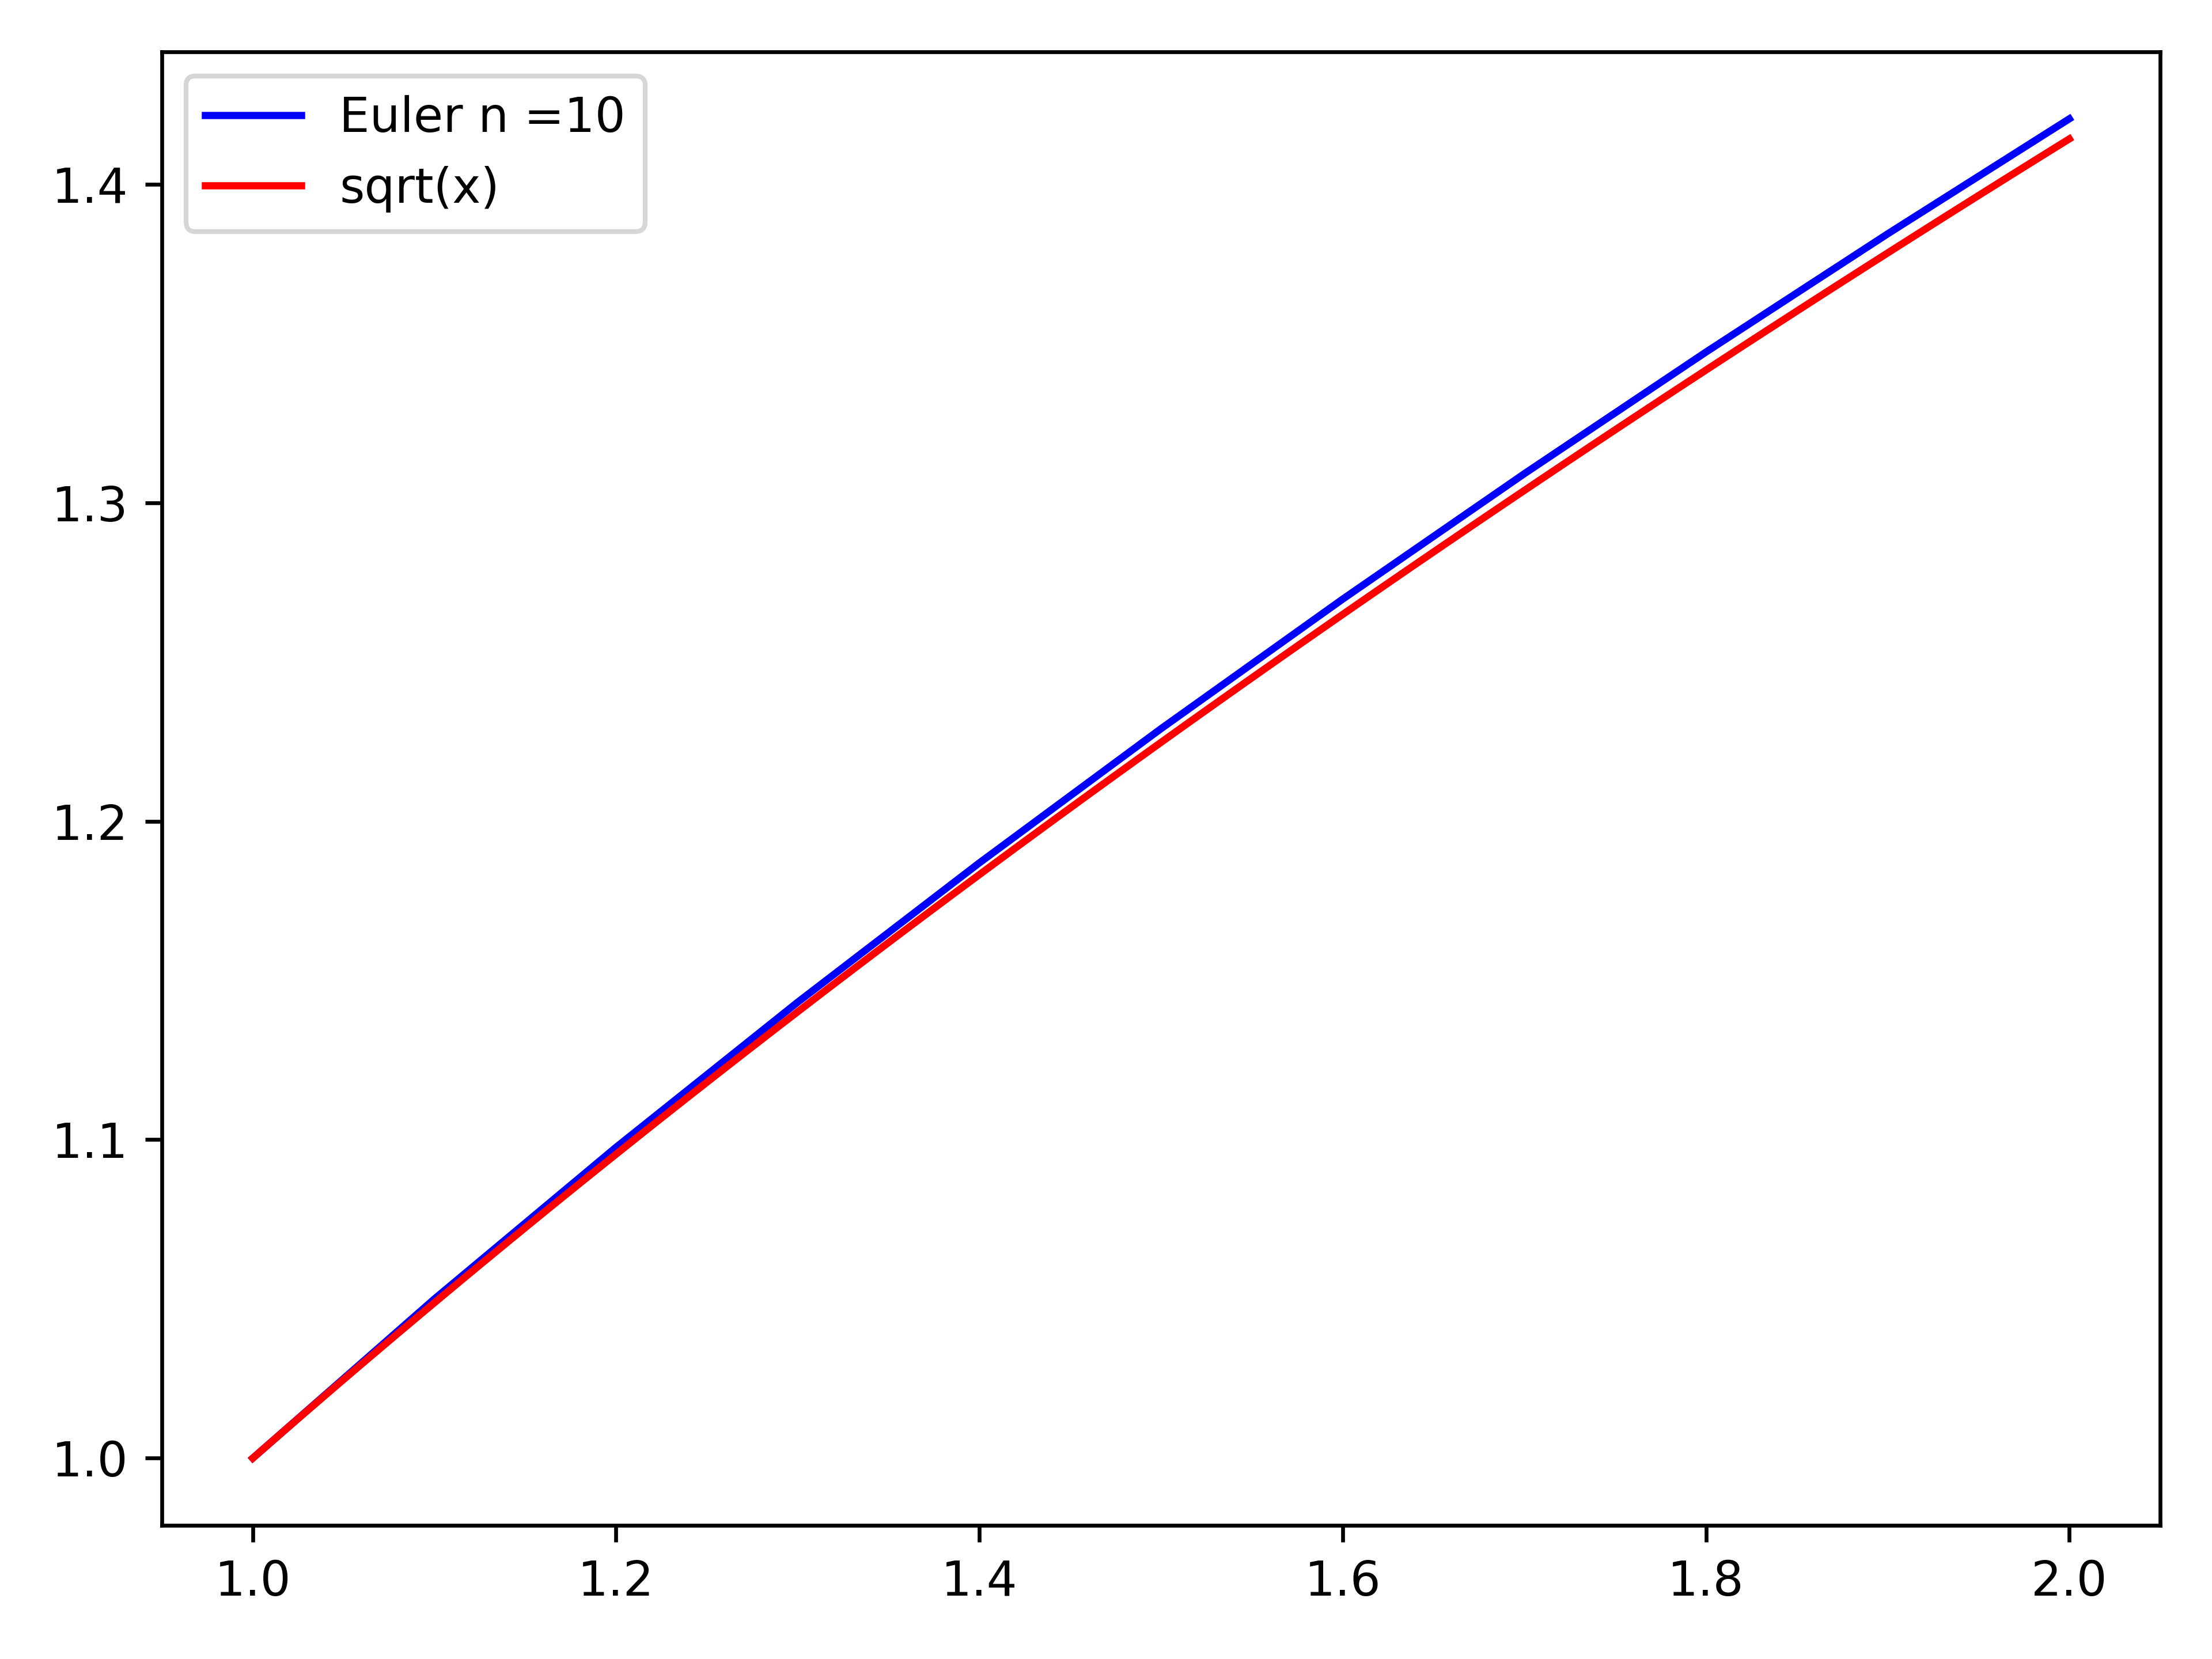
\includegraphics[scale=\myscale,scale=0.6]{figures/equadiff-euler-01}
\end{center}

Si on ne fixe pas de condition initiale, l'équation différentielle 
$$y'(x) = \frac{1}{2y(x)}$$
a une infinité de solutions $y(x) = \sqrt{x+c}$, où $c$ est une constante.
Dès que l'on fixe une condition initiale $y(x_0) = y_0$ alors la solution devient unique.
Pour quelques valeurs initiales, on trace le graphe des solutions ci-dessous.
\begin{center}
    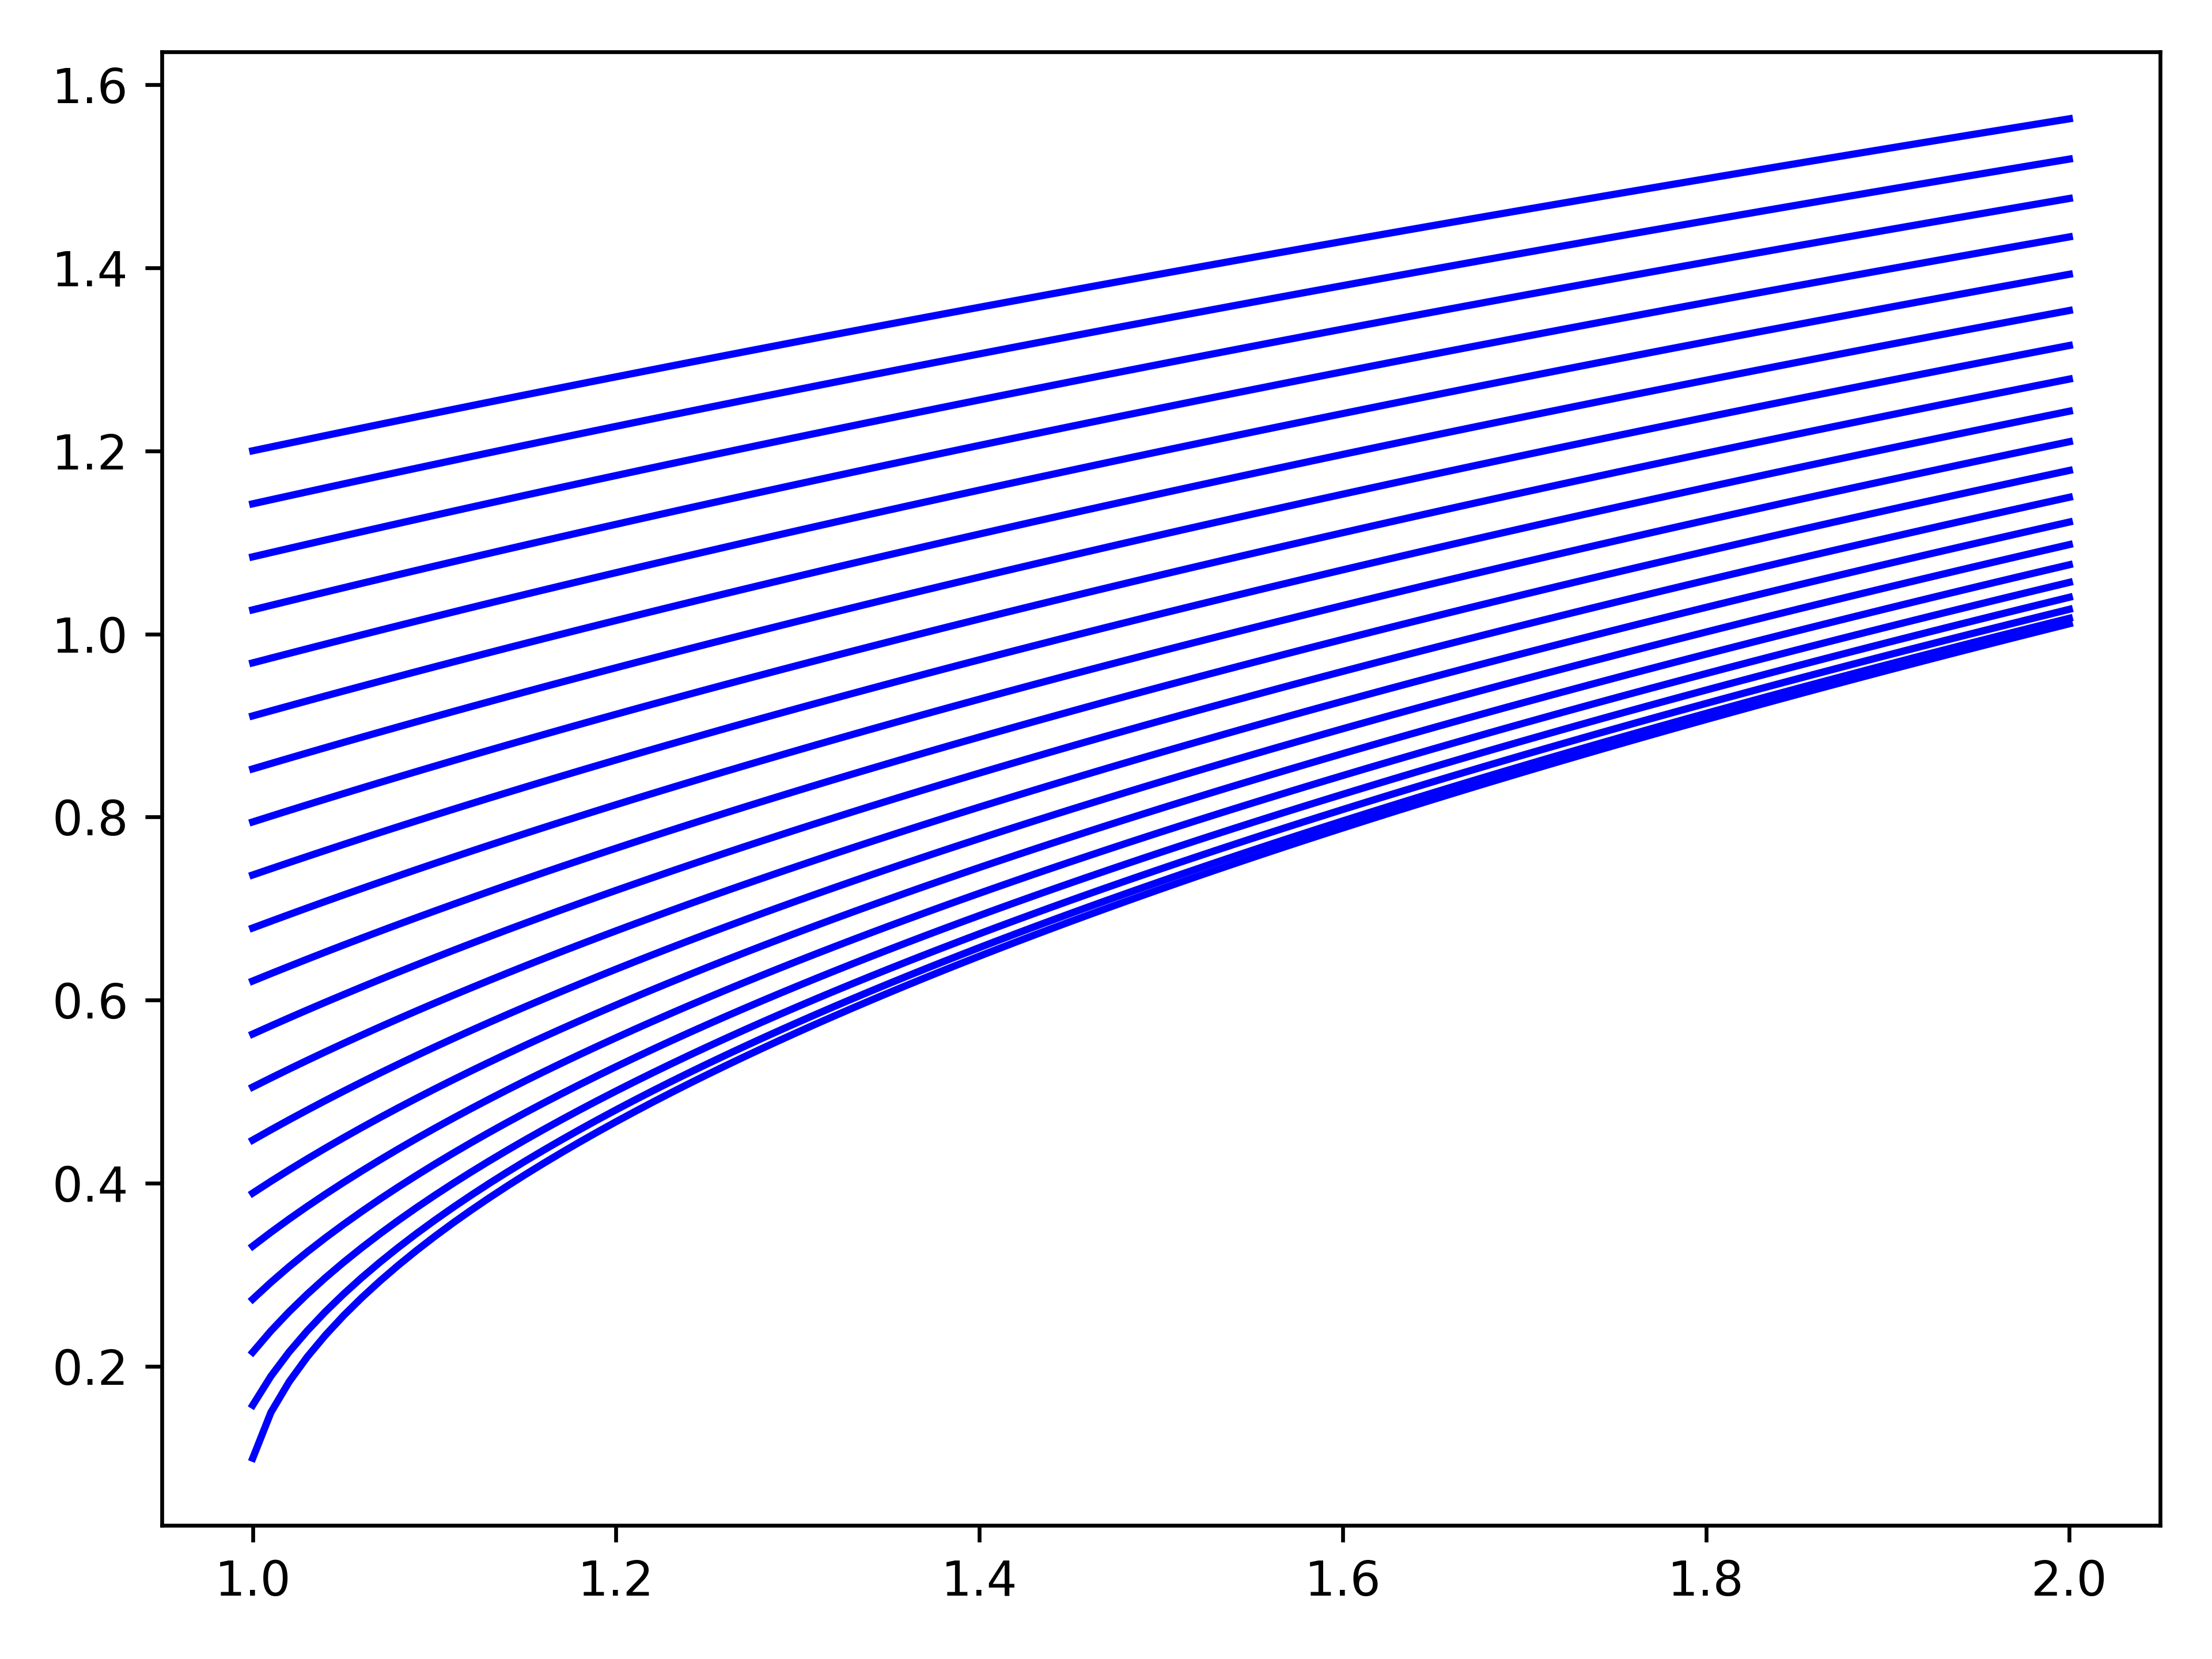
\includegraphics[scale=\myscale,scale=0.6]{figures/equadiff-euler-02}
  \end{center}
\end{exemple}

\begin{exemple}
Considérons l'équation différentielle avec une condition initiale :
$$y'(x) = y(x) \quad \text{ et } \quad y(1) = 1.$$
On trace le graphe de la solution exacte et des solutions approchées avec $n=10$ et $n=20$ subdivisions (pour $n=100$ le graphe de la solution approchée serait confondu avec le graphe de la solution exacte).
\begin{center}
  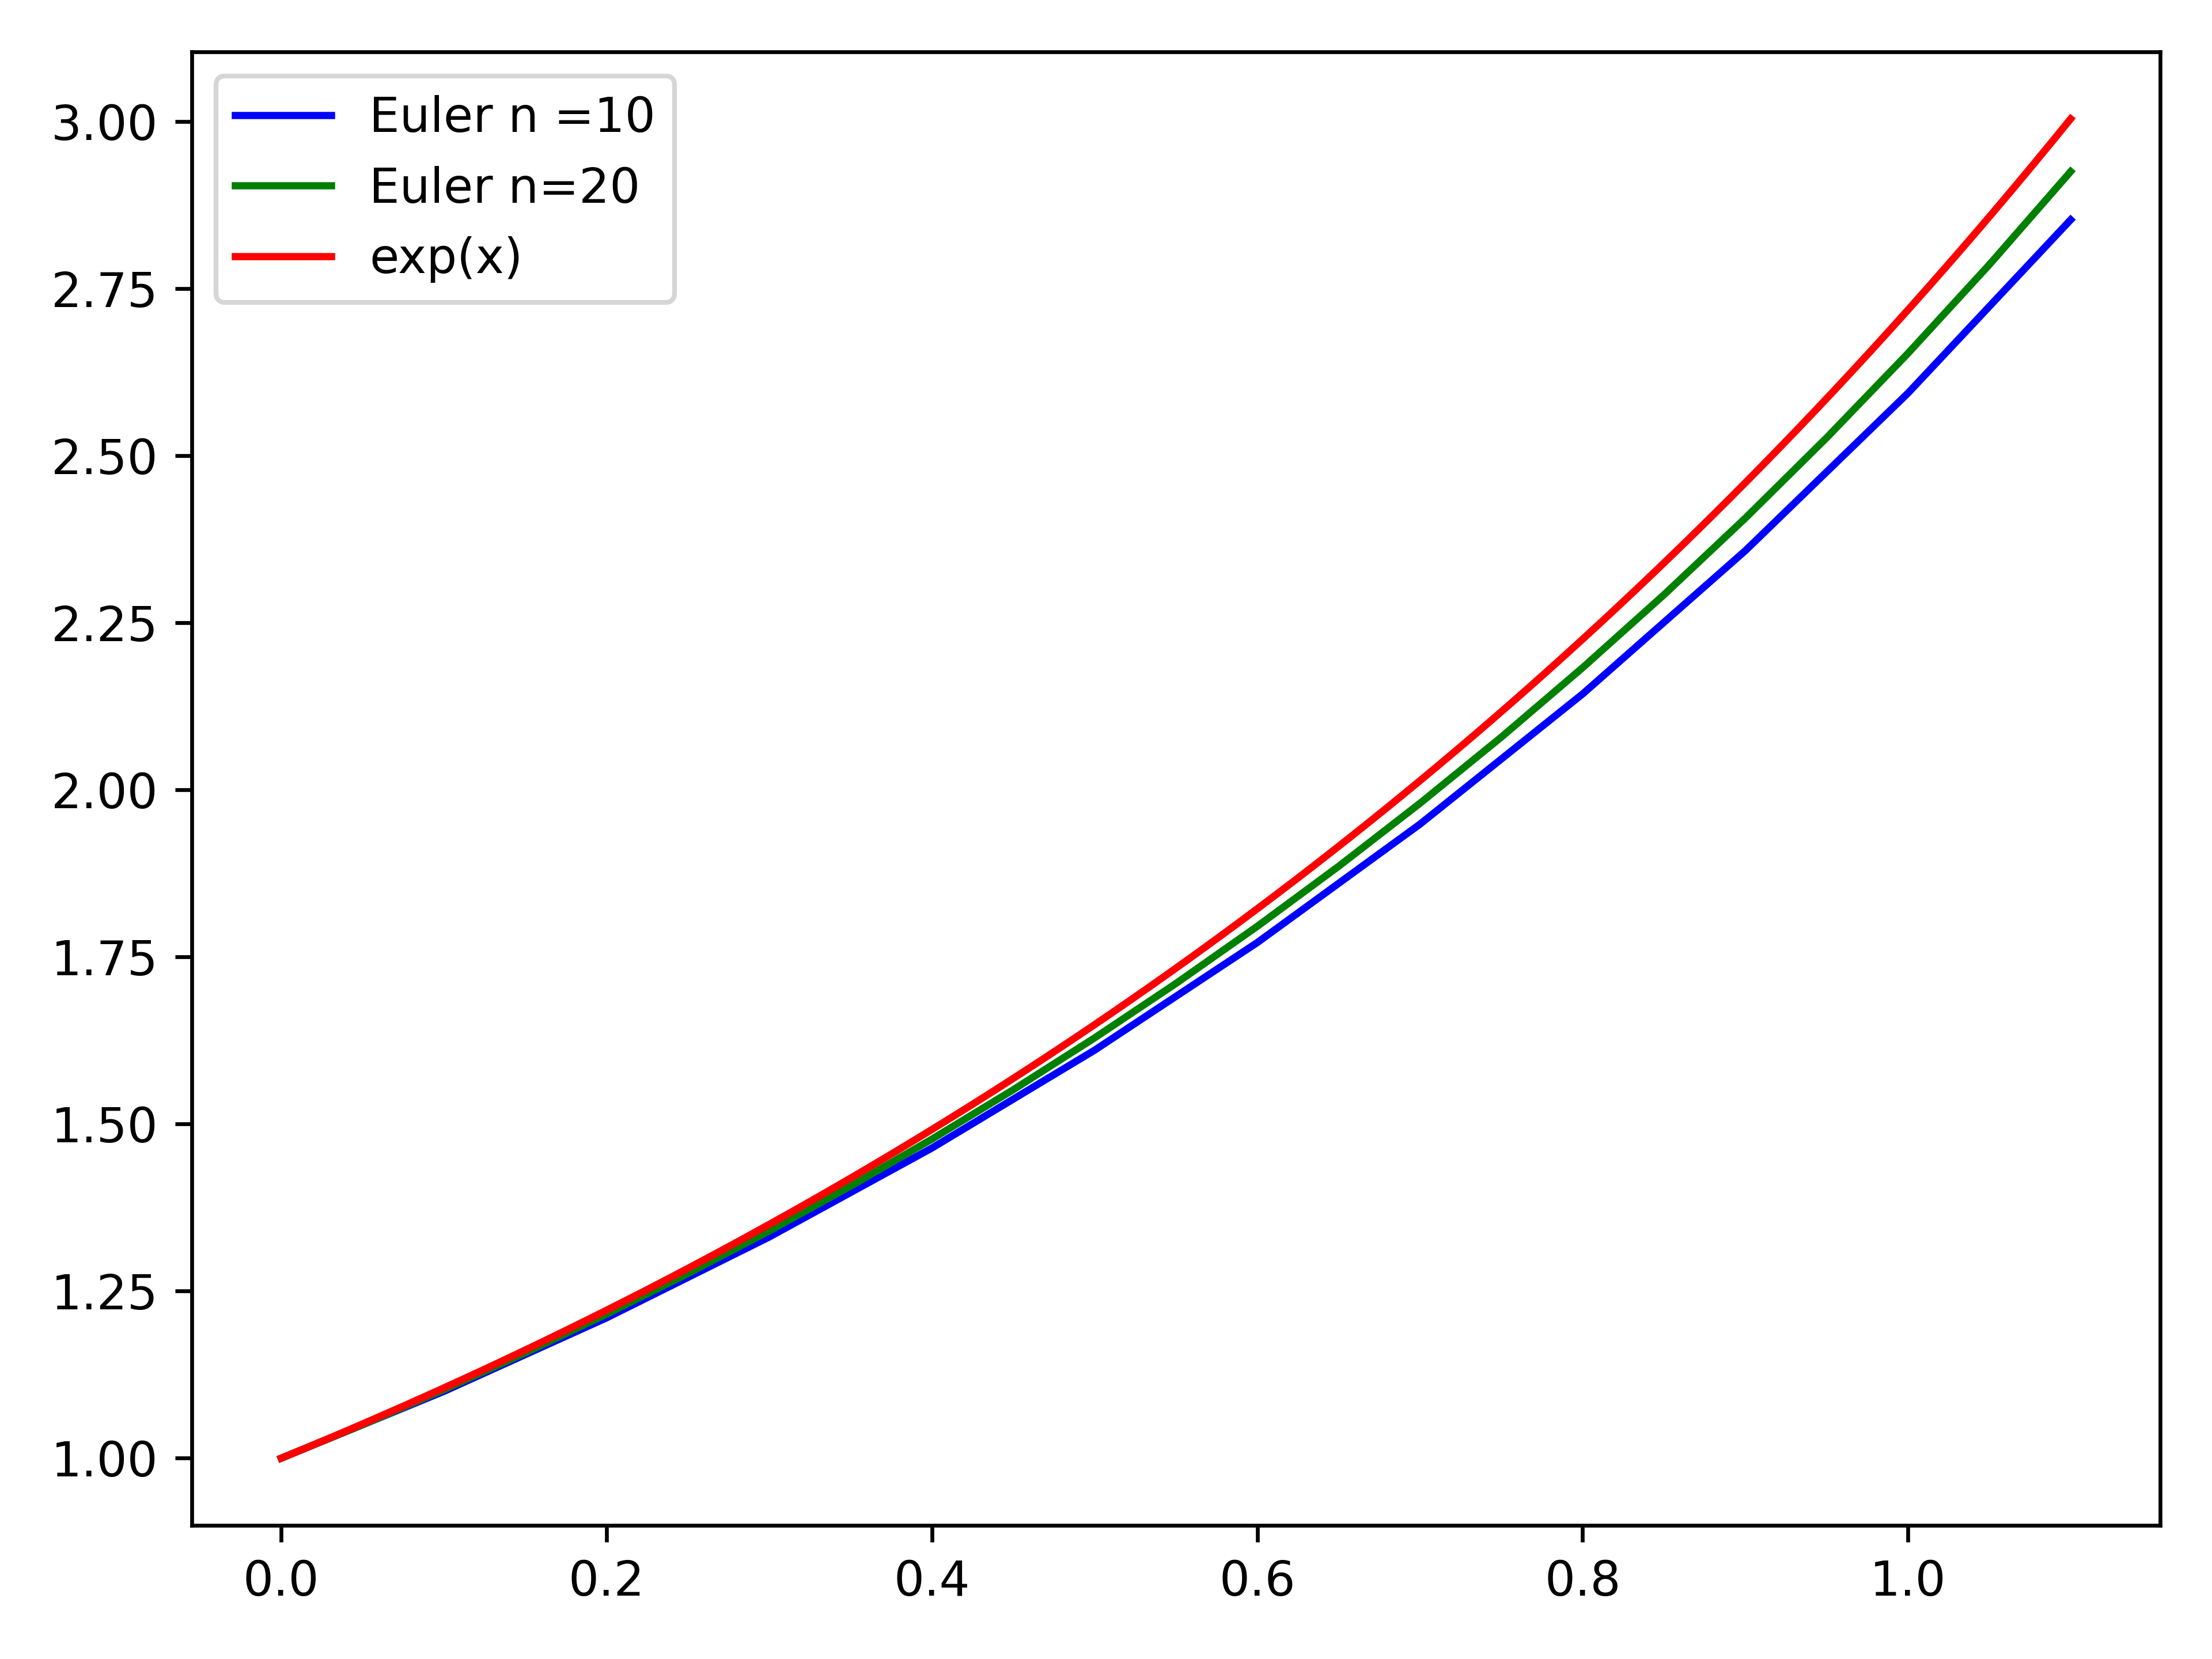
\includegraphics[scale=\myscale,scale=0.6]{figures/equadiff-euler-03}
\end{center}  
\end{exemple}



%--------------------------------------------------------------------
\subsection{Vitesse d'un parachutiste}

Déterminons la vitesse d'un parachutiste lors de son saut.
Le parachutiste est soumis à deux forces :  son poids $\vec P = m \vec g$ et la force de frottement $\vec F = - f  \| \vec v \|^2 \frac{\vec v}{\| \vec v\|}$
proportionnelle au carré de la vitesse ($f$ est le coefficient de frottement).
Le principe fondamental de la mécanique s'écrit :
$$\vec P  + \vec F = m \vec a$$
Ce qui conduit à :
$$ m g - f v^2(t) = m \frac{\dd v(t)}{\dd t}$$
Ainsi l'équation différentielle est :
$$\frac{\dd v(t)}{\dd t} = g - \frac{f}{m} v^2(t).$$
Autrement dit avec nos notations précédentes $y'(t) = g - \frac{f}{m} y^2(t)$ où $y(t)$ serait la vitesse du parachutiste.
Comme condition initiale on choisit $v(0) = 0$, c'est-à-dire qu'à l'instant initial le parachutiste démarre avec une vitesse nulle.
Il n'est pas évident de déterminer la fonction $v$ solution de cette équation différentielle. Cependant la méthode d'Euler nous fournit une solution approchée (dessinée ci-dessous pour $g=10$, $m=60$ et $f=1$).

\begin{center}
  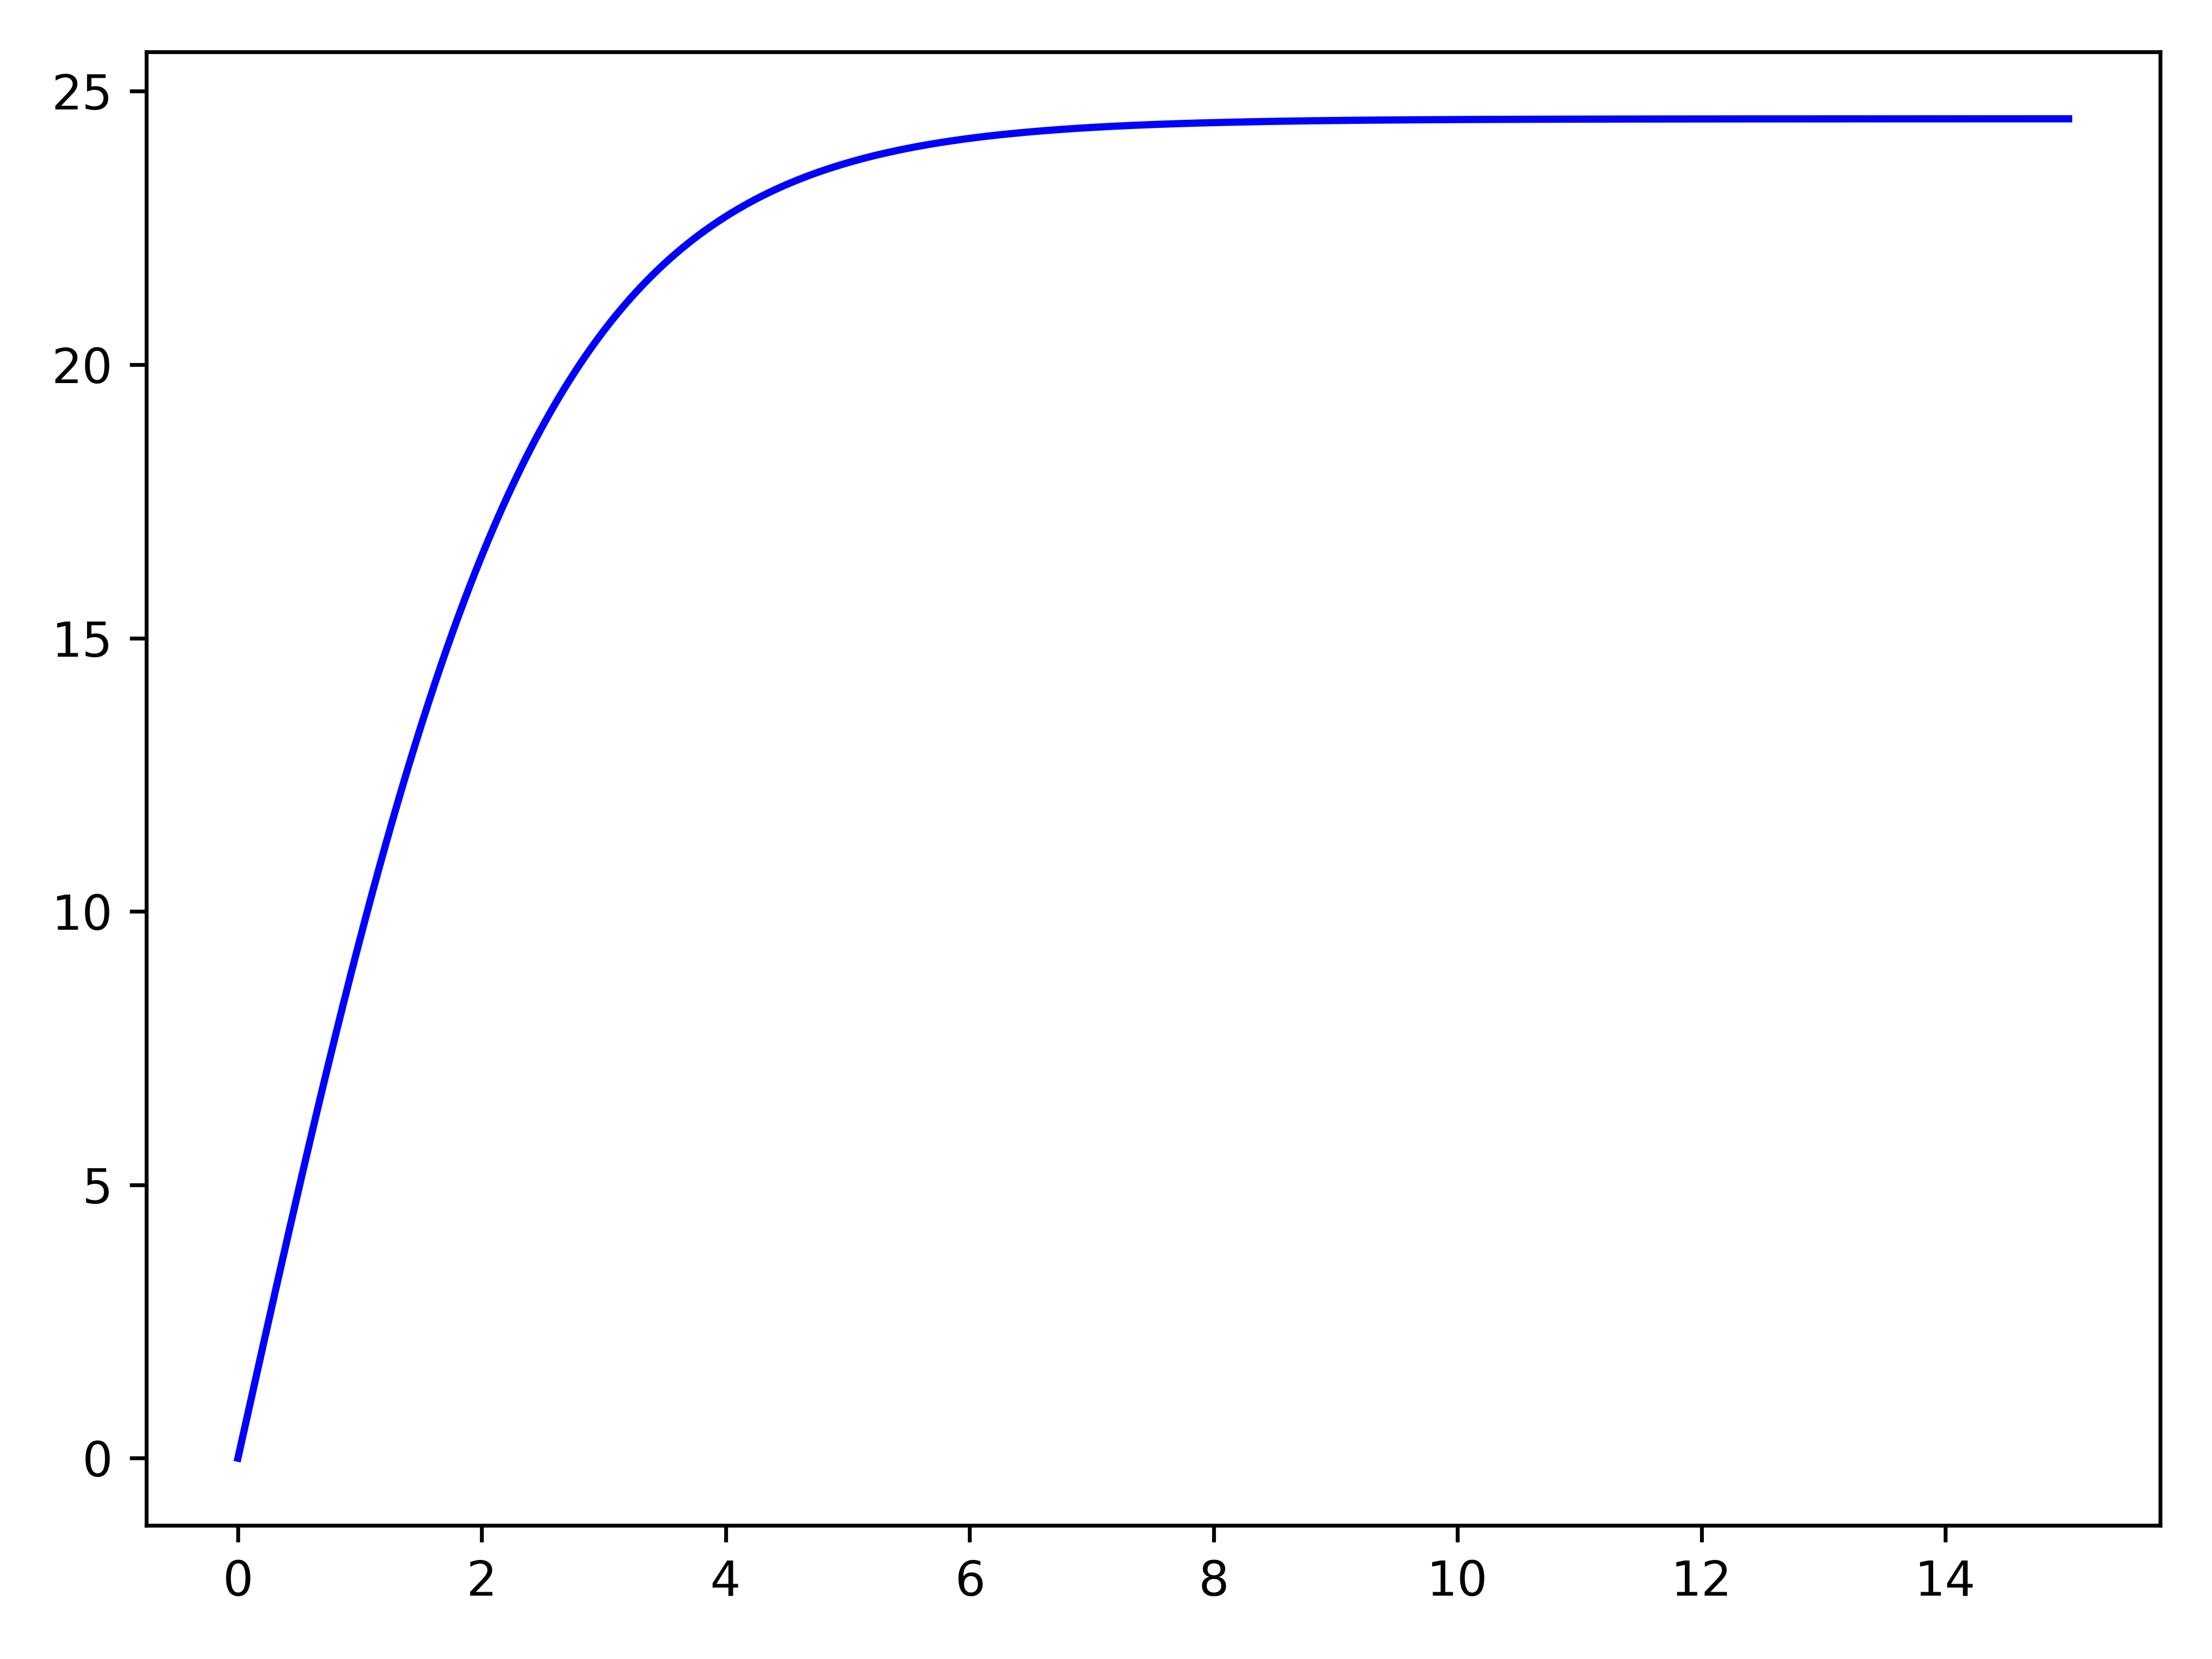
\includegraphics[scale=\myscale,scale=0.6]{figures/equadiff-euler-04}
\end{center}
La solution graphique met en évidence un phénomène vérifié expérimentalement : la vitesse augmente mais est plafonnée par une vitesse limite.

\medskip


Si on s'intéresse à la position $x$ du parachutiste (c'est-à-dire sa hauteur) cela revient à trouver une primitive de $v$, ce qui est une forme simple de résolution d'une équation différentielle :
$v(t) = \frac{\dd x(t)}{\dd t}$. On verra en fin de chapitre de tels exemples.


%%%%%%%%%%%%%%%%%%%%%%%%%%%%%%%%%%%%%%%%%%%%%%%%%%%%%%%%%%%%%%%%%%%%%
\section{Méthodes de Runge-Kutta}

\index{algorithme!methode de Runge-Kutta@méthode de Runge-Kutta}

%--------------------------------------------------------------------
\subsection{Retour sur la méthode d'Euler}

Expliquons graphiquement un pas de la méthode d'Euler.
On se place en $x_n$, on suppose connue (ou estimée) la valeur $y_n$ de la fonction $y$ en $x_n$.
L'équation différentielle nous donne la valeur de la dérivée $y'(x_n)$ en $x_n$.
On trace la tangente à la courbe $y(x)$ en $x_n$, c'est-à-dire la droite passant par le point $(x_n,y_n)$ et de pente $y'(x_n)=f(x_n,y_n)$.
On considère que la tangente approche bien la courbe $y(x)$ sur un petit intervalle $[x_n,x_n+h]$, donc la valeur de $y(x)$ sur cet intervalle est approximativement donnée par la tangente, en particulier :
$$y(x_n+h) \simeq y_n + h y'(x_n).$$

\myfigure{1}{
	\tikzinput{fig-equadiff-euler}
}  



La méthode d'Euler itère ce processus, autrement dit, on obtient une formule de récurrence, initialisée par $x_0$ et $y_0$, puis :
$$
\left\lbrace
\begin{array}{rcl}
  x_{n+1} &=& x_n + h \\  
  y_{n+1} &=& y_n + h f(x_n,y_n)
\end{array}
\right.
$$





%--------------------------------------------------------------------
\subsection{Runge-Kutta d'ordre 2}

Pour la méthode de Runge-Kutta d'ordre 2 (RK2), chaque pas se fait en deux étapes préalables, puis un calcul de moyenne :
\begin{enumerate}
  \item On calcule d'abord la pente de la tangente au point de départ $k_1 = f(x_n,y_n)$.
  On en déduit une approximation de la valeur de $y$ en $x_n+h$, c'est-à-dire $y_n+h k_1$.
  
  \item On calcule ensuite la pente de la tangente au point d'arrivée : $k_2 = f(x_n+h,y_n+h k_1)$.

  \item On prend pour valeur de $y$ en $x_n+h$ la valeur correspondant à la moyenne des ces deux pentes : $y_{n+1} = y_n + \frac{h}{2} (k_1 + k_2)$.
\end{enumerate}

La méthode de Runge-Kutta d'ordre 2 itère ce processus.
La formule combinant ces étapes est :
$$y(x_n+h) \simeq y_n + \frac{h}{2} \Big(  f(x_n,y_n) + f(x_n+h, y_n + h f(x_n,y_n))\Big).$$

La formule de récurrence est :
$$
\left\lbrace
\begin{array}{rcl}
    k_1 &=& f(x_n,y_n) \\
    k_2 &=& f(x_n + h, y_n + h k_1) \\
    x_{n+1} &=& x_n + h \\
    y_{n+1} &=& y_n + \frac h2 (k_1 + k_2) \\
\end{array}
\right.
$$

\myfigure{1}{
	\tikzinput{fig-equadiff-rk2}
} 

Pourquoi cette méthode est-elle meilleure que la méthode d'Euler ? La méthode d'Euler est basée sur la tangente au point initial et fait partir l'approximation franchement au-dessus ou en-dessous du graphe de la solution. Par contre avec la méthode de Runge-Kutta d'ordre 2, la direction suivie combine la pente au départ et à l'arrivée et est beaucoup plus proche de la solution exacte.
On fera une comparaison numérique entre les méthodes dans une section suivante.
Il existe une variante de la méthode de Runge-Kutta d'ordre 2 ou la pente utilisée est la pente calculée en $x_n + \frac{h}{2}$.


Si on fait une analogie avec le calcul approché d'intégrale : la méthode d'Euler s'apparente à la méthode des rectangles, 
la méthode RK2 avec la méthode des trapèzes, 
la méthode RK4 avec la méthode de Simpson.

\myfigure{1}{
	\tikzinput{fig-int-01}
} 

\myfigure{0.7}{
	\tikzinput{fig-int-02}\qquad
	\tikzinput{fig-int-03}\qquad
	\tikzinput{fig-int-04}		
} 

%--------------------------------------------------------------------
\subsection{Runge-Kutta d'ordre 4}

La méthode de Runge-Kutta d'ordre 4 (RK4) est encore plus précise que la méthode d'ordre 2. C'est l'une des méthodes les plus populaires.
La formule est obtenue à l'aide d'une moyenne pondérée de quatre pentes de tangentes.
Voici sa formule de récurrence $x_{n+1} = x_n+h$ et :
$$y_{n+1} = y_n + \frac h6 \left( k_1 + 2 k_2 + 2 k_3 + k_4 \right)$$
avec :
$$
\left\lbrace  
\begin{array}{rcl}
  k_1 &=& f(x_n,y_n) \\
  k_2 &=& f(x_n + \frac h2, y_n + \frac h2 k_1) \\
  k_3 &=& f(x_n + \frac h2, y_n + \frac h2 k_2) \\
  k_4 &=& f(x_n + h, y_n + h k_3)
\end{array}
\right.
$$

\myfigure{1}{
	\tikzinput{fig-equadiff-rk4}
} 


%--------------------------------------------------------------------
\subsection{Comparaisons}

À chaque étape nos méthodes font des approximations. Plus le pas $h$ est petit, plus l'erreur commise est petite.
Ces erreurs se cumulent lors des itérations. On peut donc comparer les méthodes en fonction de l'erreur commise à chaque étape et de l'erreur totale commise à la fin de l'itération.
Voici un tableau des ordres de grandeurs des ces erreurs :

\begin{center}
\begin{tabular}{c|c|c}
Méthode & erreur locale & erreur globale \\
\hline
Euler & $O(h^2)$ & $O(h)$ \\
RK2 & $O(h^3)$ & $O(h^2)$  \\
RK4 & $O(h^5)$ & $O(h^4)$  \\
\end{tabular}
\end{center}

Ainsi, si $h=0.1$ l'erreur totale commise par la méthode d'Euler est de l'ordre de $0.1$, celle de la méthode RK2 est de l'ordre de $0.01$ et celle de la méthode RK4 est de l'ordre de $0.0001$. On voit donc que les méthodes RK2 et RK4 sont beaucoup plus précises que la méthode d'Euler.
Il faut cependant noter que la méthode RK2 évalue la fonction $f$ deux fois à chaque étape et est donc deux fois plus lente que la méthode d'Euler, mais 
comme l'erreur est quadratique en $h$, le gain de précision est substantiel.

Voici les valeurs numériques pour le calcul de $\sqrt{2}$ obtenu comme la valeur en $2$ de la solution de l'équation différentielle $y'=\frac1{2y}$ avec $y(1)=1$. En gras sont indiquées les décimales exactes.

\begin{center}
\begin{tabular}{c|c|c|c}
pas & Euler & RK2 & RK4 \\
\hline
$h=0.1$ 
& \textbf{1.4}20519799291044
& \textbf{1.41421}57109943851
& \textbf{1.4142135}76569407 \\
$h=0.01$
& \textbf{1.414}8279673659128
& \textbf{1.41421356}44527205
& \textbf{1.41421356237}4446 \\
\end{tabular}
\end{center}



Sur le graphe ci-dessous on dessine les solutions exactes et approchées du problème $y'(x)=y(x)$ avec $y(0)=1$ pour un pas $h=0.1$.
Les méthodes de Runge-Kutta sont si efficaces que l'on n'arrive pas à distinguer le graphe de la solution exacte ($y(x) = e^x$) avec les solutions approchées RK2 et RK4.

\begin{center}
  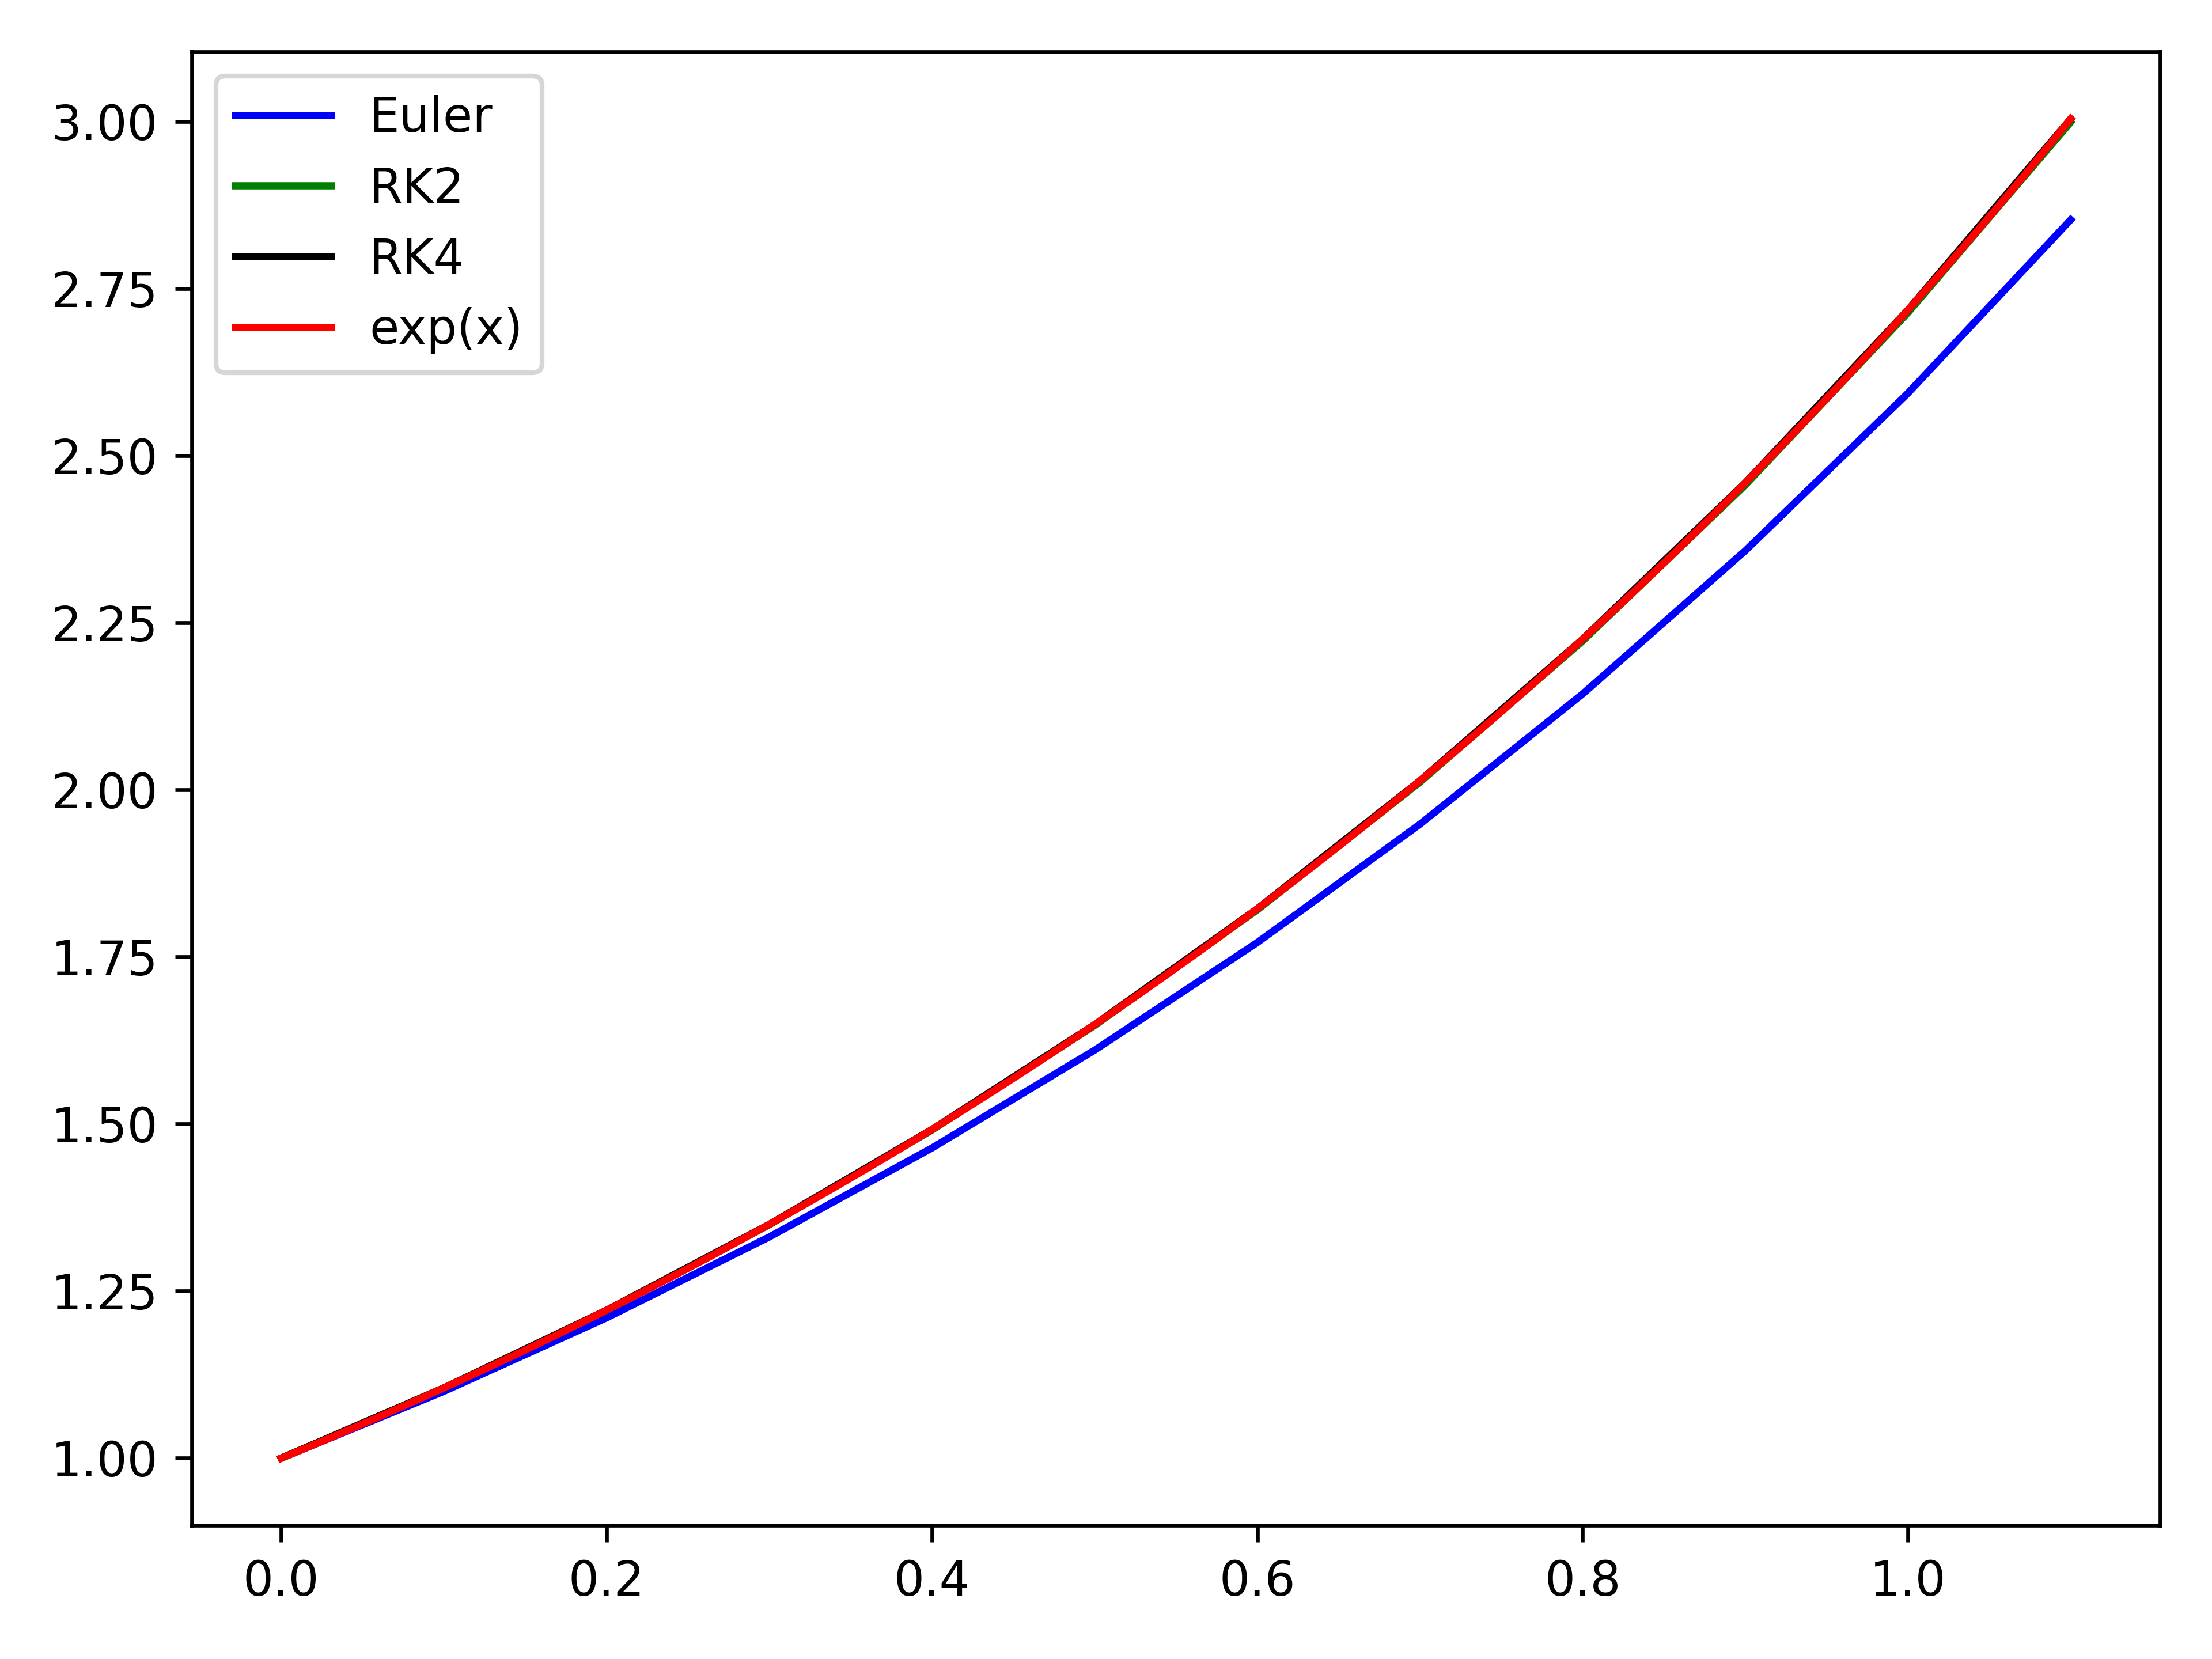
\includegraphics[scale=\myscale,scale=0.7]{figures/equadiff-euler-05}
\end{center}


%%%%%%%%%%%%%%%%%%%%%%%%%%%%%%%%%%%%%%%%%%%%%%%%%%%%%%%%%%%%%%%%%%%%%
\section{Systèmes d'équations différentielles}

%--------------------------------------------------------------------
\subsection{Intégration des champs de vecteurs}

Un \defi{champ de vecteurs} est la donnée pour chaque point $(x,y) \in \Rr^2$ du plan d'un vecteur $\vec F (x,y)$.

Ci-dessous le champ de vecteurs $\vec F (x,y) = (y, -x)$.
\begin{center}
  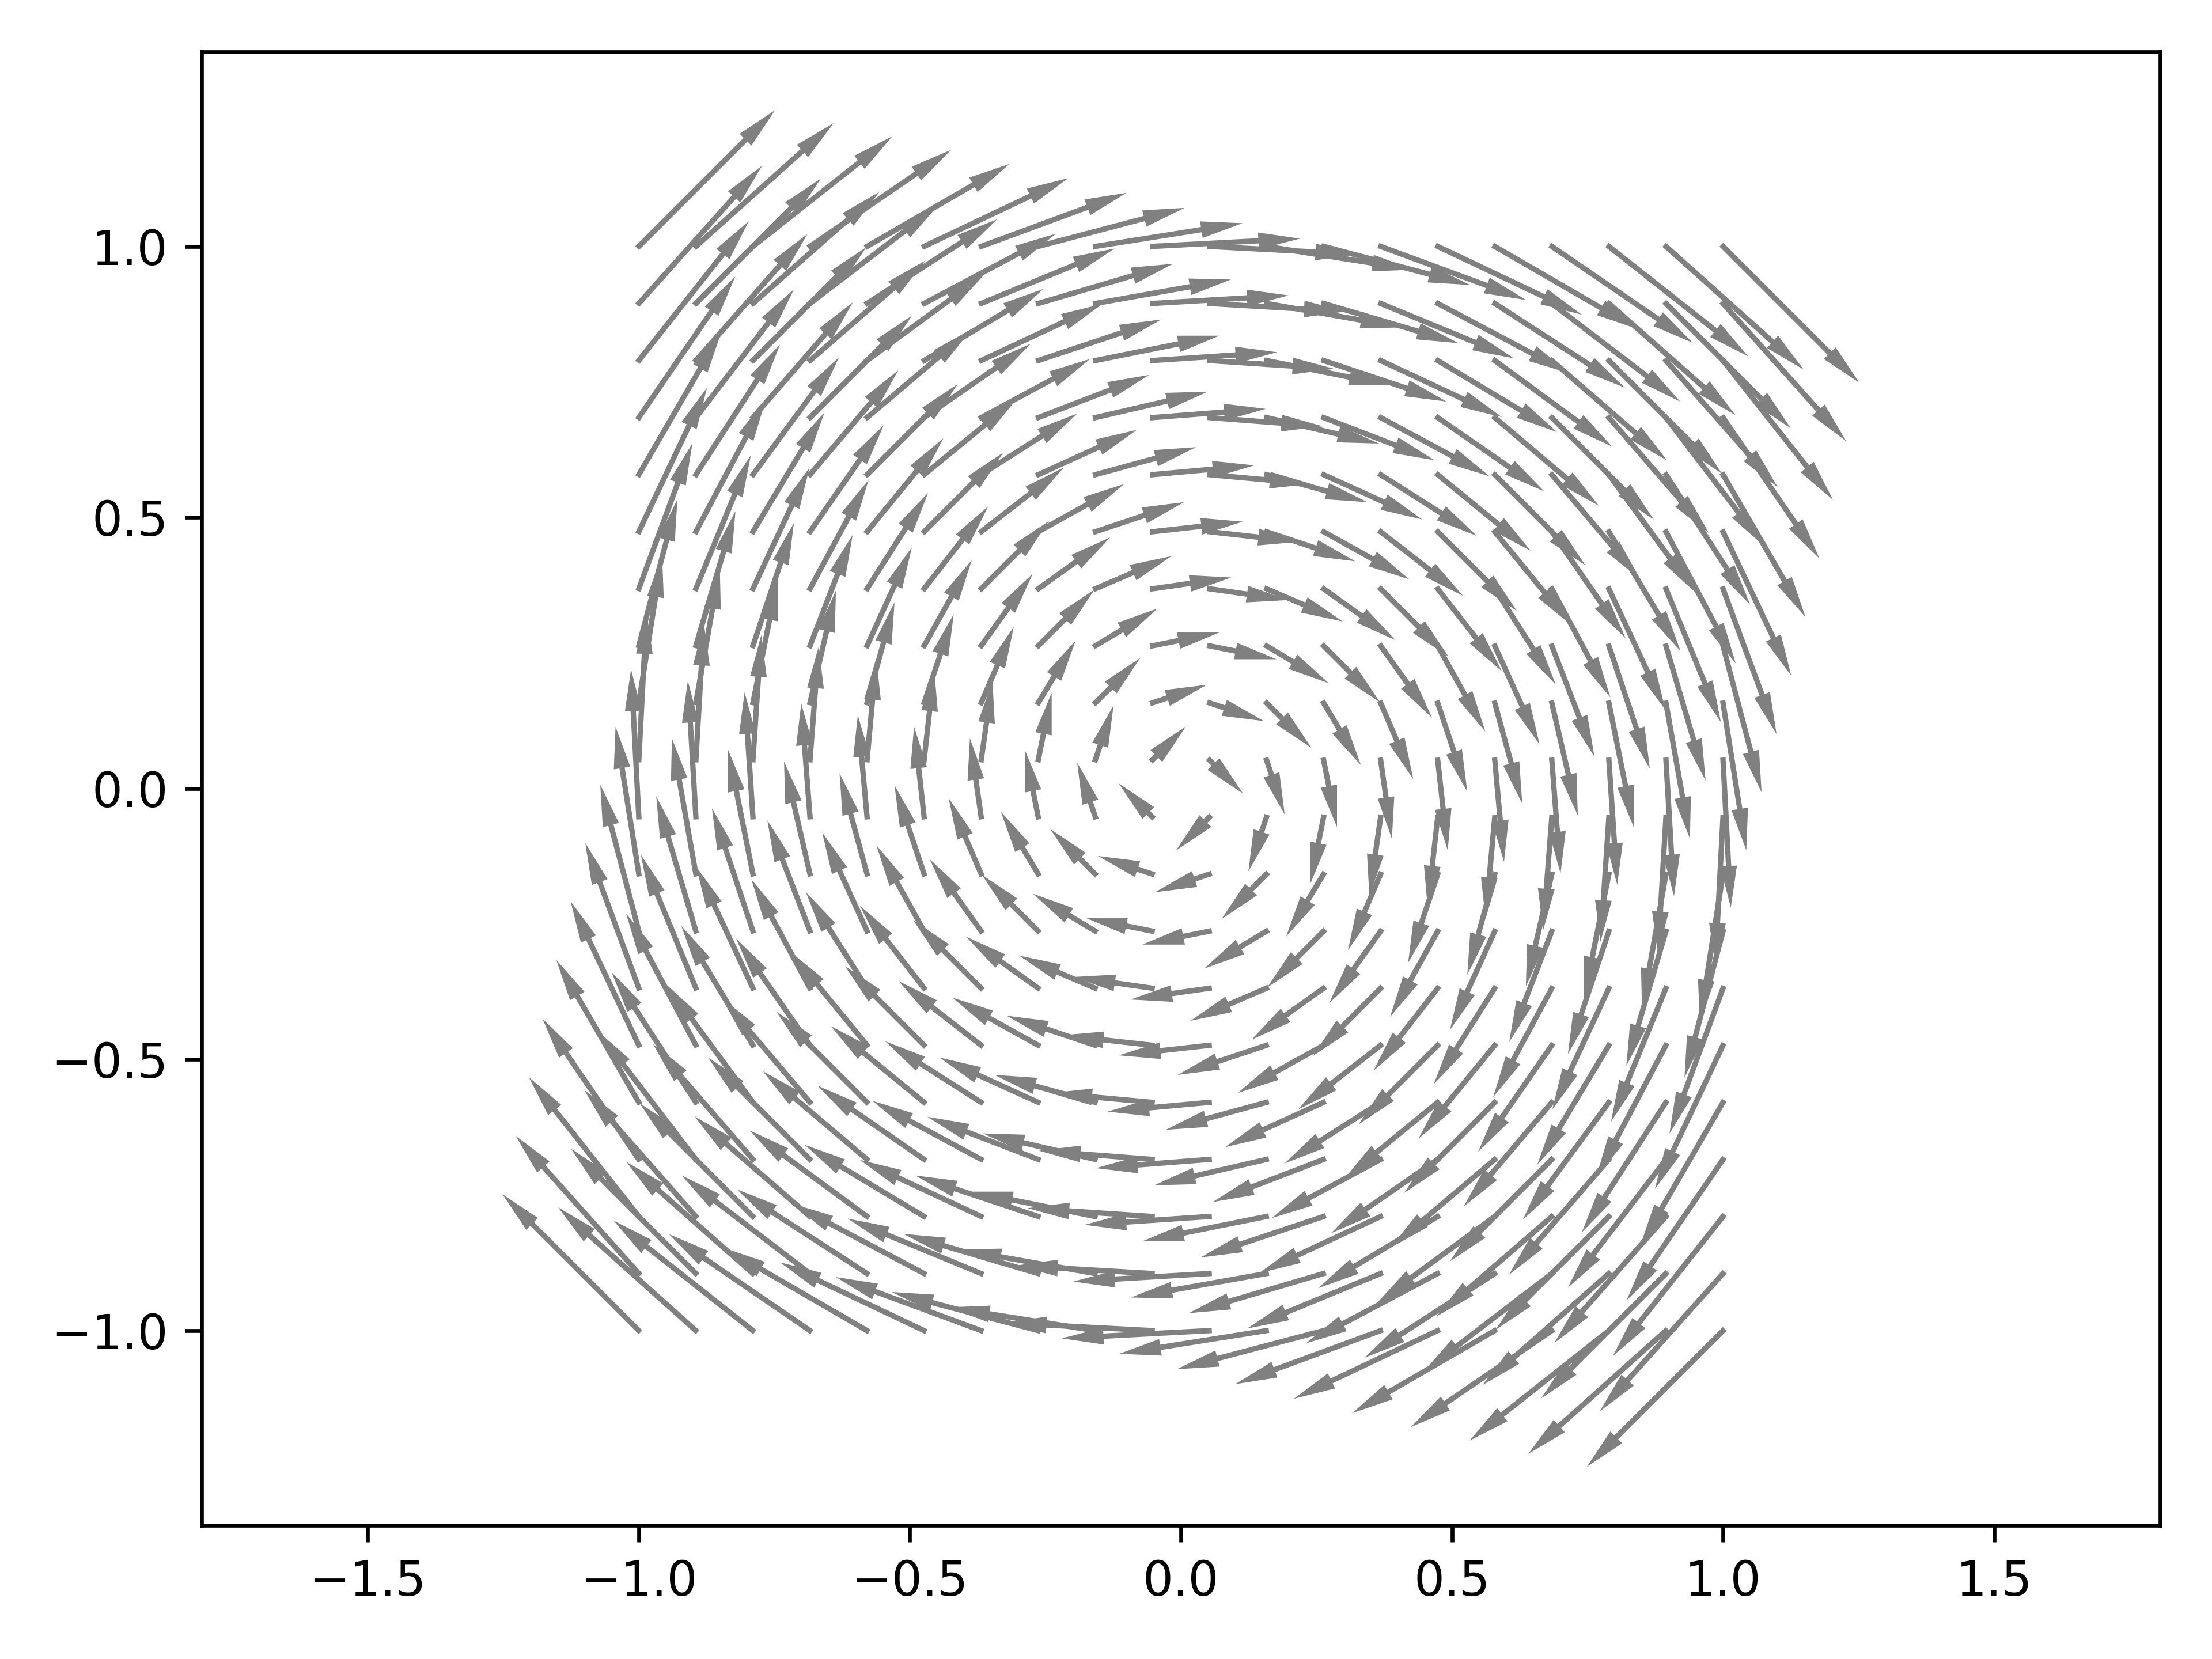
\includegraphics[scale=\myscale, scale=0.7]{figures/equadiff-sys-01}
\end{center}

Une \defi{courbe intégrale} est un arc $\gamma(t) = (x(t), y(t) )$ tel que pour tout $t \in \Rr$ :
$$(x'(t), y'(t)) = \vec F(x,y).$$
Si on note $\vec F (x,y) = (f(x,y), g(x,y))$ alors cela revient à trouver une solution du système différentiel suivant :
$$\left\lbrace
\begin{array}{rcl}
  x'(t) &=& f(x(t),y(t)) \\
  y'(t) &=& g(x(t),y(t))
\end{array}
\right.$$


Graphiquement, en partant d'une position initiale $(x_0,y_0)$, la courbe intégrale correspond à suivre les flèches du champ de vecteurs.
Ci-dessous : une portion d'une courbe intégrale (à gauche), les courbes intégrales sont en fait des paramétrisations de cercles (à droite).
\begin{center}
  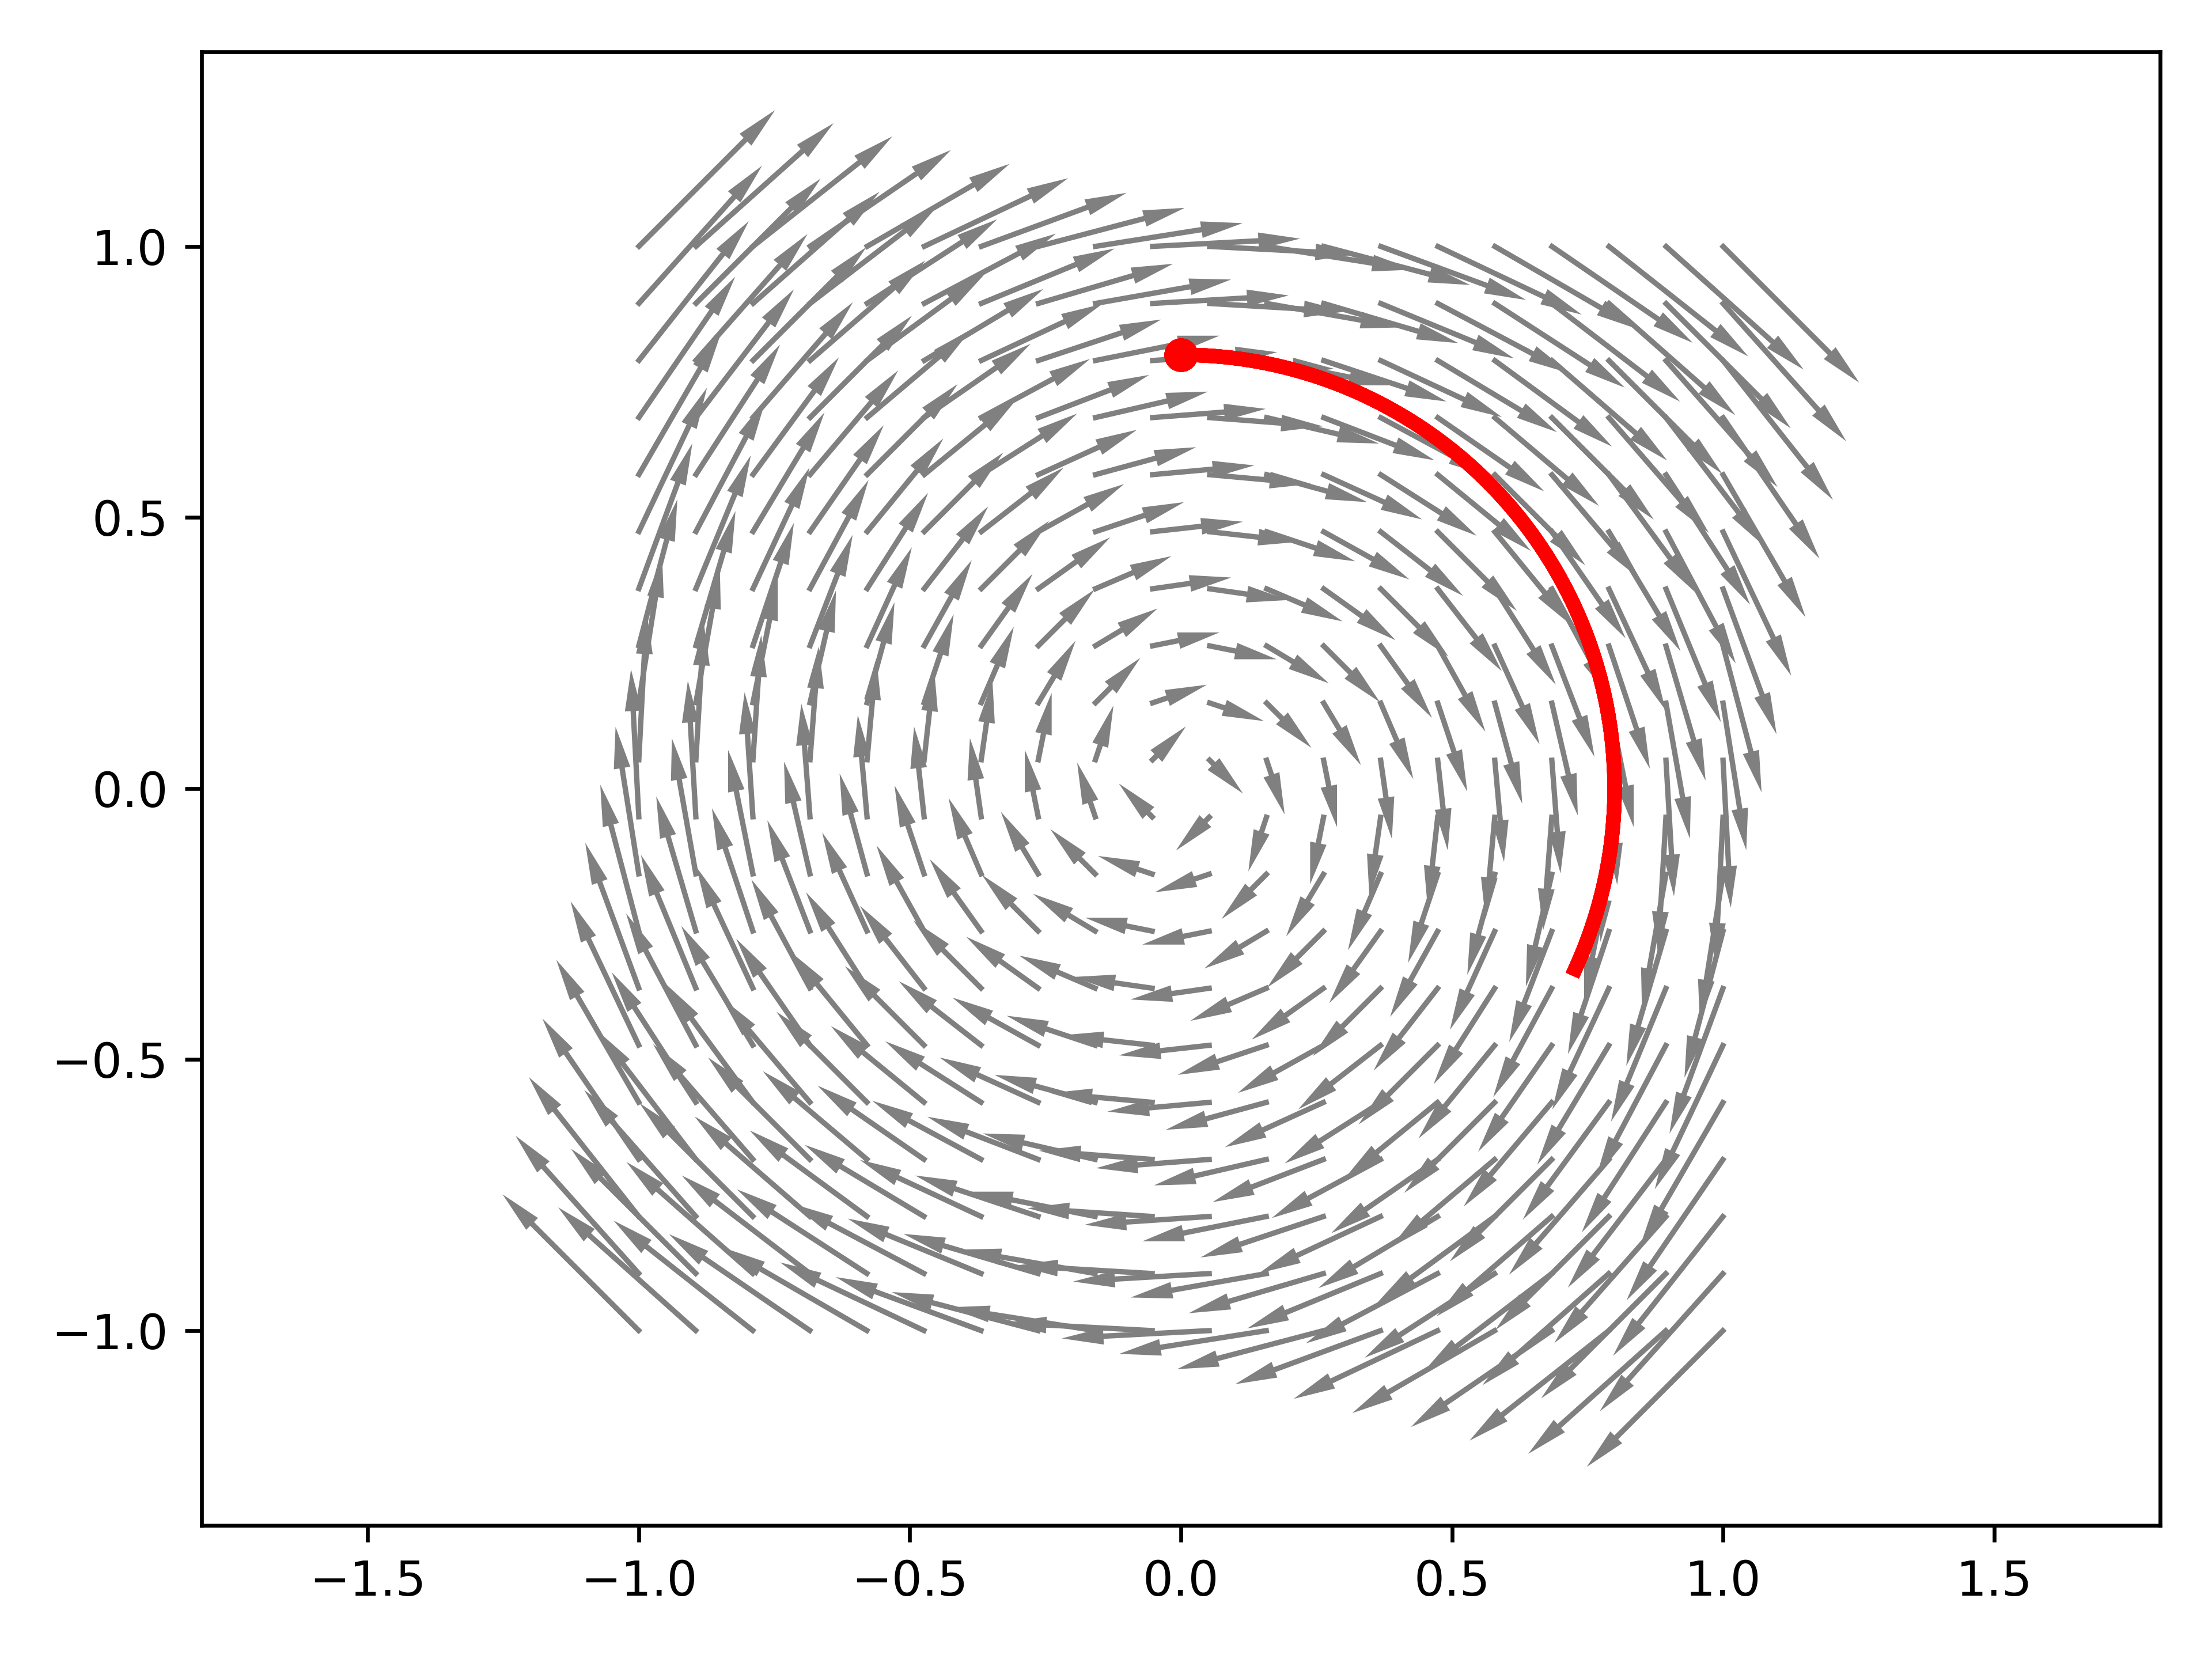
\includegraphics[scale=\myscale, scale=0.5]{figures/equadiff-sys-02}\qquad
  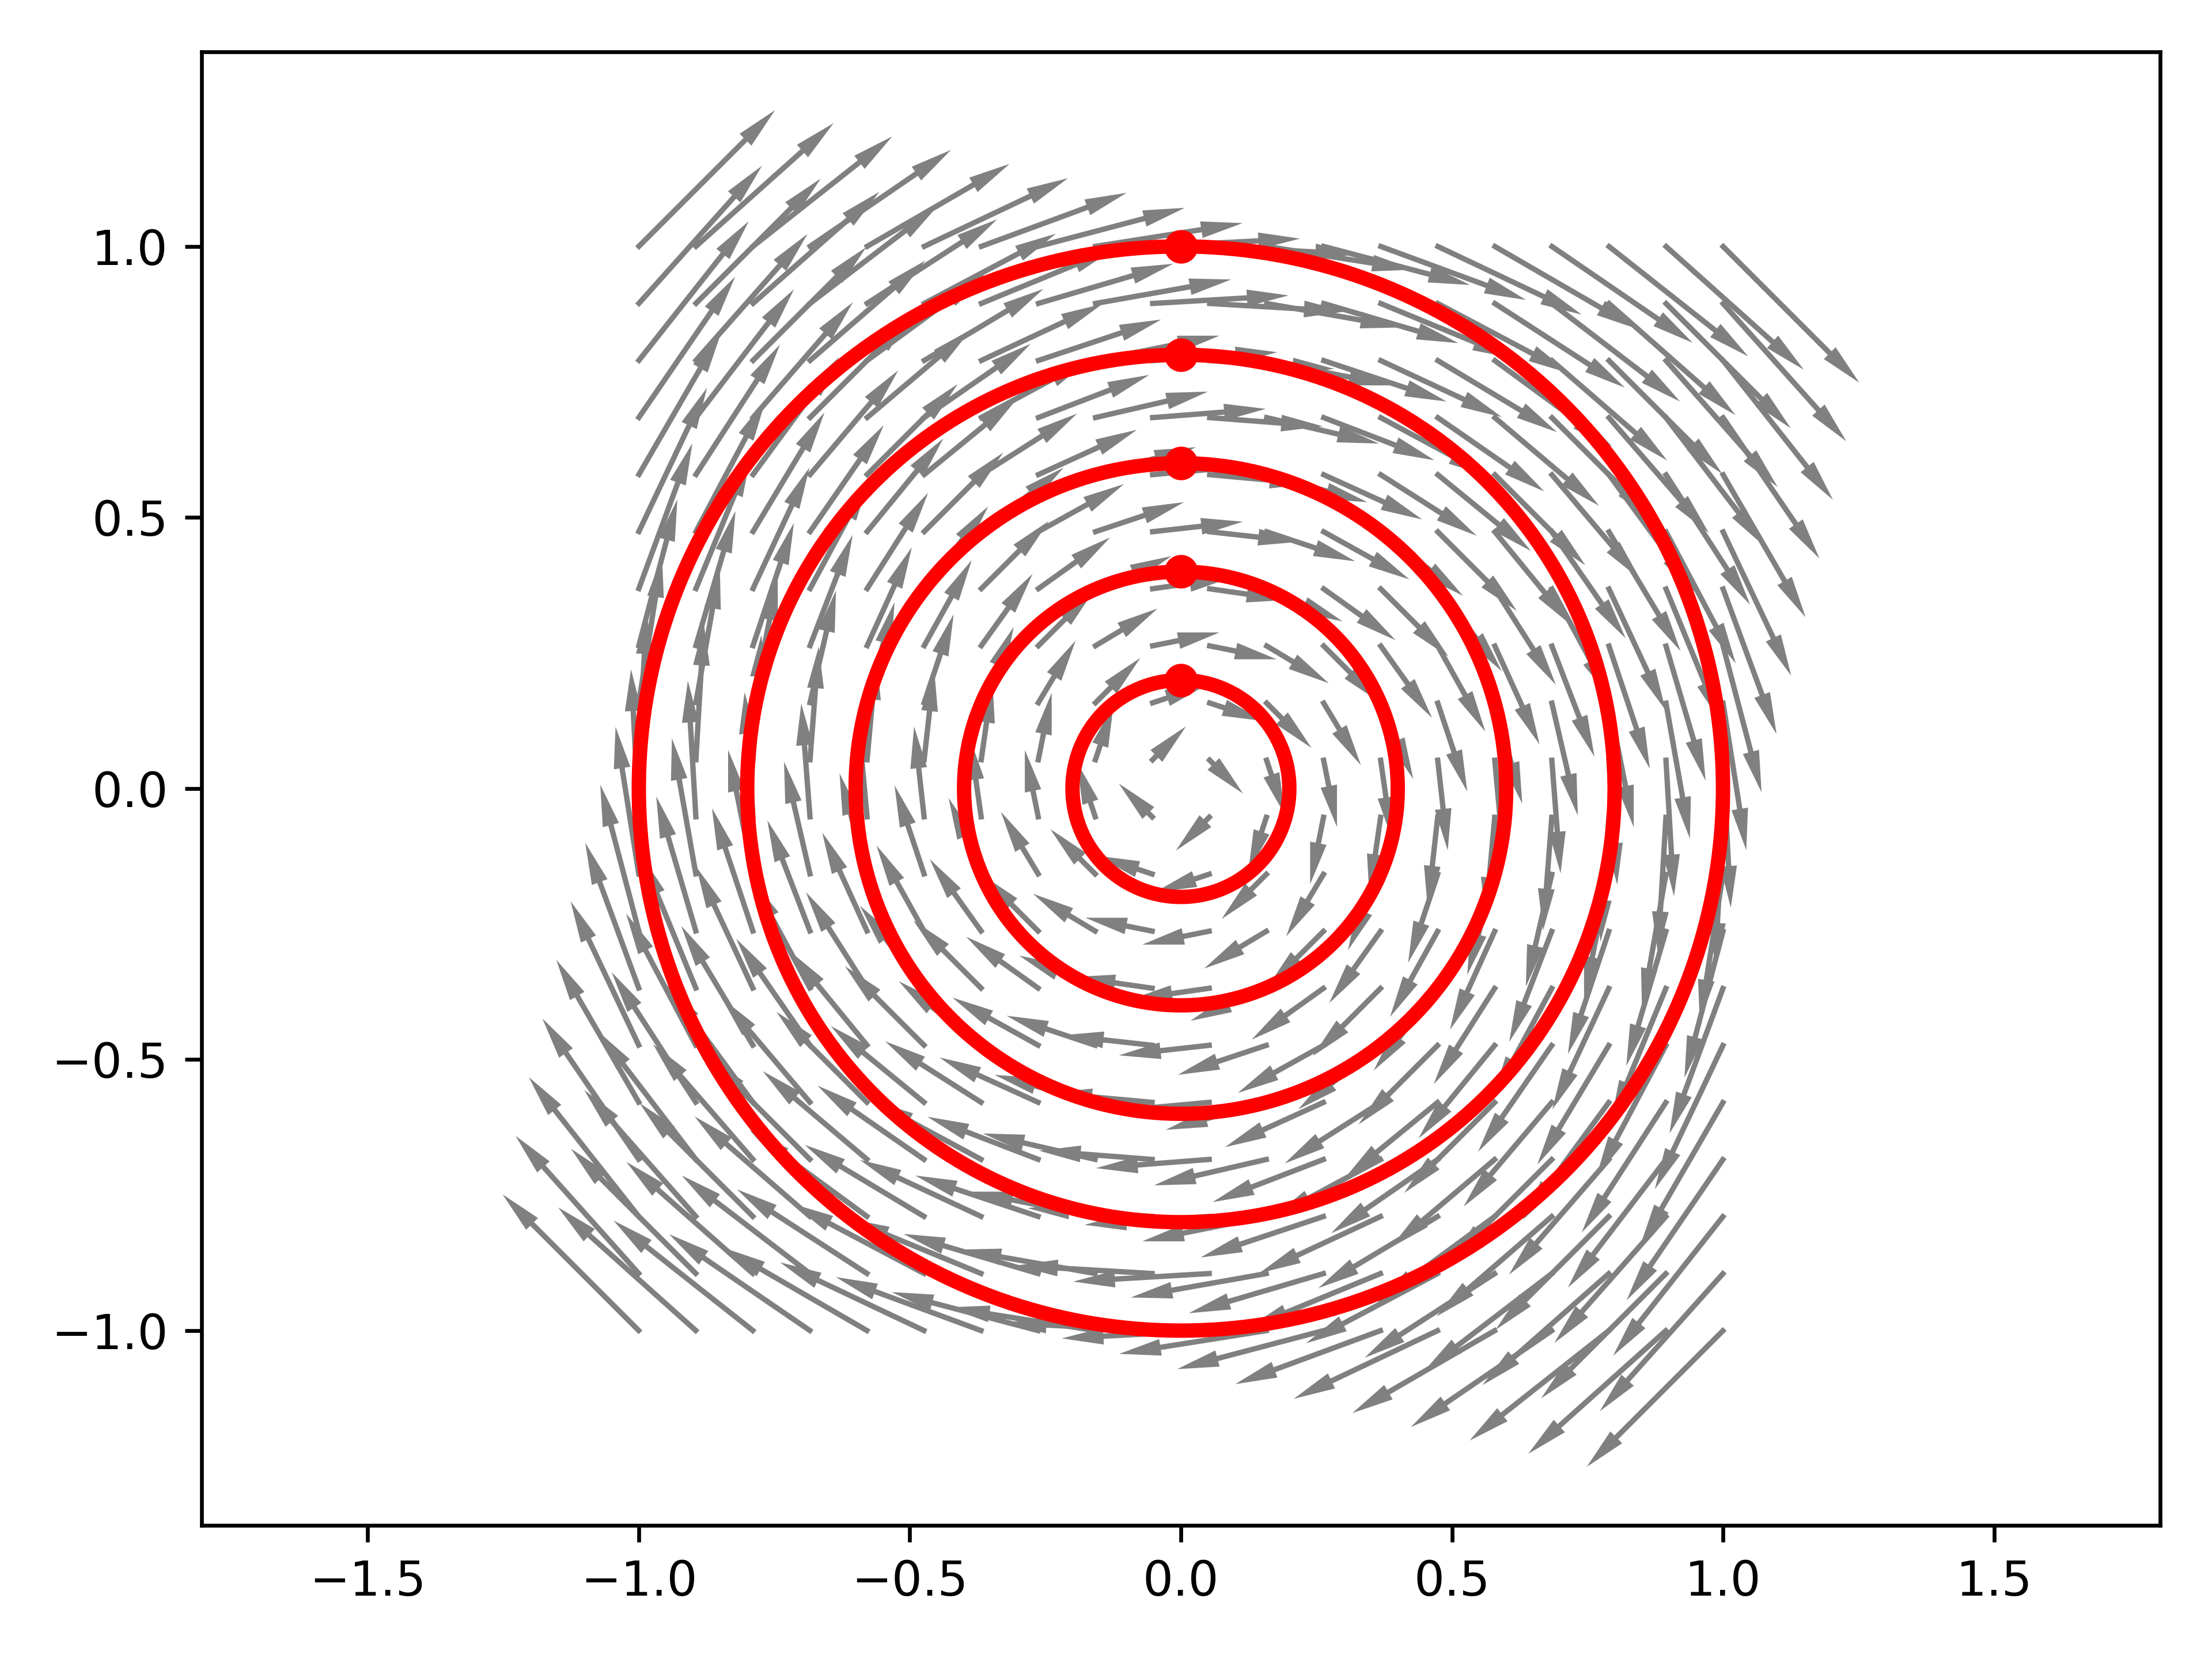
\includegraphics[scale=\myscale, scale=0.5]{figures/equadiff-sys-03} 
\end{center}


\bigskip

La méthode d'Euler s'étend sans difficulté à ce cas.

\textbf{Méthode d'Euler.}

Soit $x_0,y_0 \in \Rr$ et $h>0$.
$$\left\lbrace
\begin{array}{rcl}
  x_{n+1} &=& x_n + h f(x_n,y_n) \\
  y_{n+1} &=& y_n + h g(x_n,y_n)  
\end{array}
\right.$$

\bigskip

Voici la méthode de Runge-Kutta d'ordre 2.

\textbf{Méthode RK2.}

Soit $x_0,y_0 \in \Rr$ et $h>0$.
$$\left\lbrace
\begin{array}{rcl}
  k_1 &=& f(x_n,y_n) \\
  \ell_1 &=& g(x_n,y_n) \\
  k_2 &=& f(x_n + h k_1, y_n + h \ell_1) \\
  \ell_2 &=& g(x_n + h k_1, y_n + h \ell_1) \\
  x_{n+1} &=& x_n + \frac{h}{2} (k_1 + k_2) \\
  y_{n+1} &=& y_n + \frac{h}{2} (\ell_1 + \ell_2)
\end{array}
\right.$$

\bigskip

Voici un autre exemple de champ de vecteurs : $\vec F (x,y) = (x-y, xy)$.
\begin{center}
  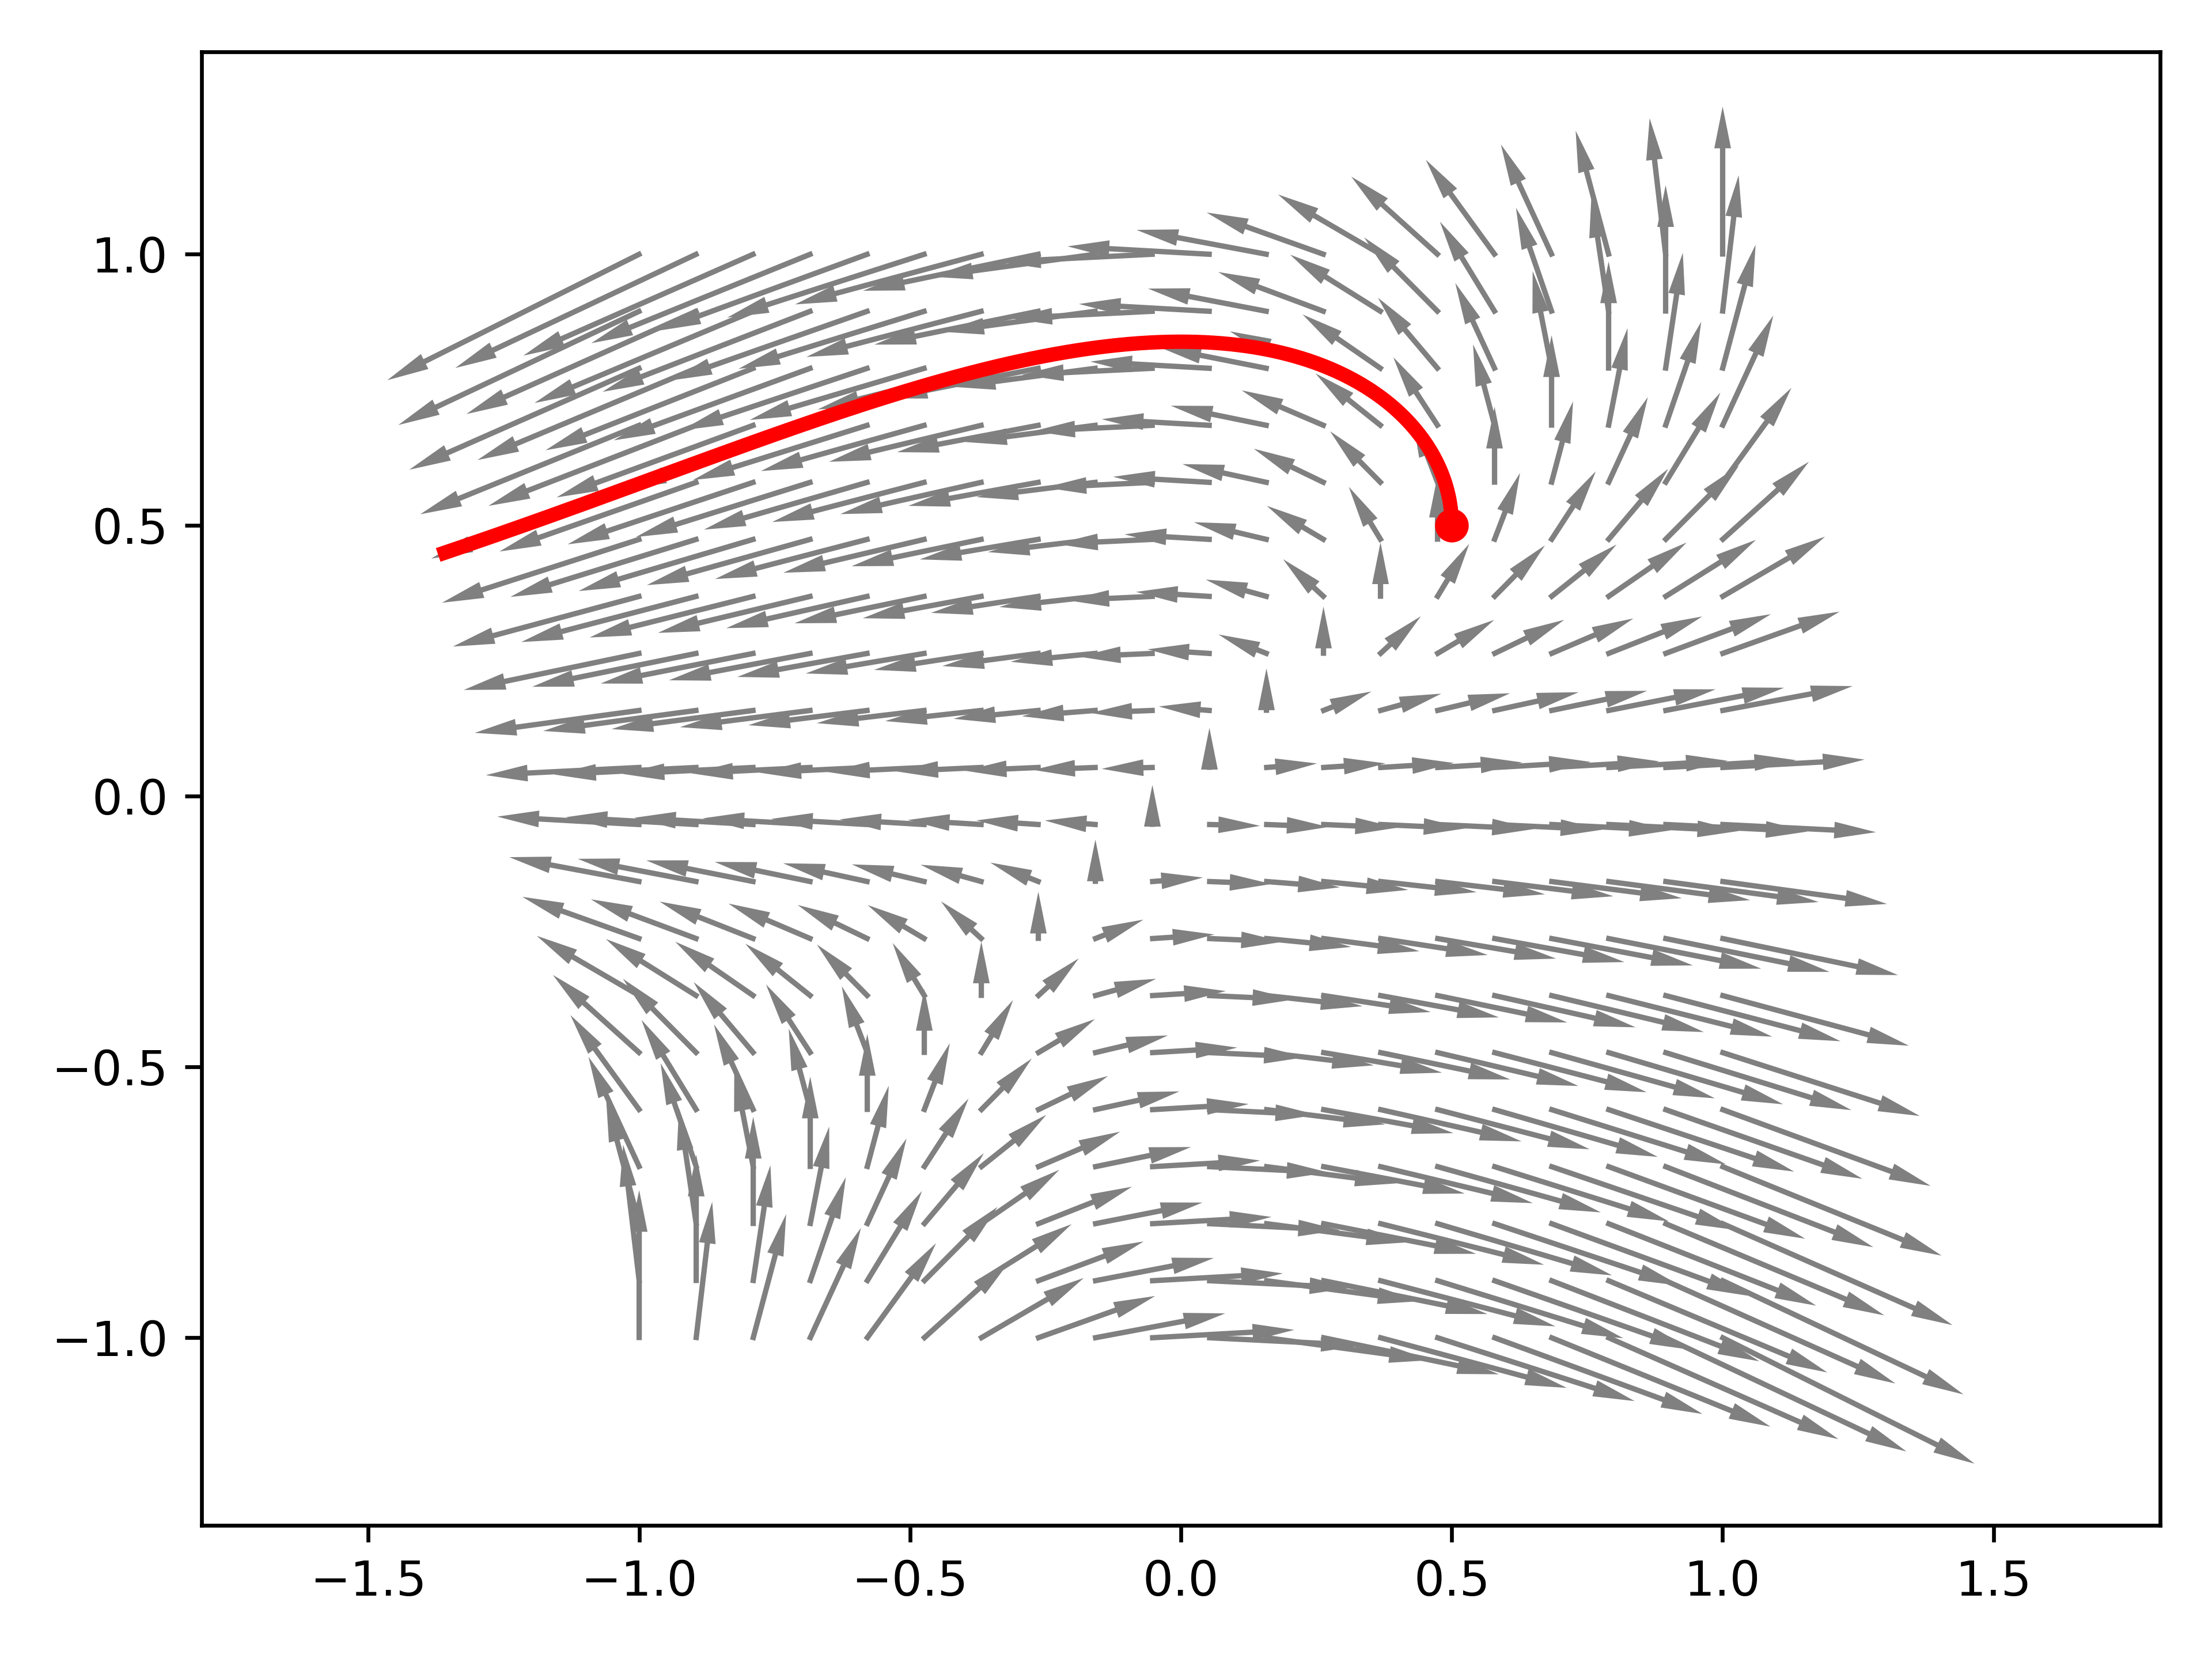
\includegraphics[scale=\myscale, scale=0.8]{figures/equadiff-sys-04}
\end{center}


%--------------------------------------------------------------------
\subsection{Équations différentielles d'ordre 2}

Considérons une équation différentielle d'ordre $2$, c'est-à-dire faisant intervenir $y(x)$, $y'(x)$ et $y''(x)$ :
$$y''(x) = f(x,y,y').$$
Elle se transforme en un système de deux équations différentielles d'ordre $1$. On pose $z(x) = y'(x)$ et on a alors :
$$\left\lbrace
\begin{array}{rcl}
  y'(x) &=& z(x) \\
  z'(x) &=& f(x,y,z)
\end{array}
\right.$$
La solution est généralement unique une fois que l'on a fixé les conditions initiales $y(x_0)$ et $y'(x_0)$. On peut alors appliquer les méthodes numériques précédentes.


\bigskip

Le principe fondamental de la mécanique conduit naturellement à un système d'équations différentielles d'ordre $2$. En effet la vitesse est la dérivée de la position et l'accélération est la dérivée seconde de la position.

Appliquons ceci au mouvement d'un satellite orbitant dans le plan orbital de la Terre et du Soleil (supposés tous les deux fixes !). Le satellite est soumis à la force d'attraction de la Terre et à celle du Soleil.
Ces forces s'écrivent :
$$\vec{F_T} = - \frac{G m M_T}{r_T^2} \vec{e_T}
\qquad
\vec{F_S} = - \frac{G m M_S}{r_T^2} \vec{e_S}$$
et le principe fondamental de la mécanique donne :
$$\vec{F_T} + \vec{F_S} = m \vec a$$
Les données sont :
\begin{itemize}
  \item $m$ : masse du satellite,
  \item $M_T$ : masse de la Terre,
  \item $M_S$ : masse du Soleil,
  \item $G$ : constante gravitationnelle,
  \item $r_T$ : distance du satellite à la Terre,
  \item $r_S$ : distance du satellite au Soleil,
  \item $\vec e_T$ : vecteur unitaire issu de la Terre dans la direction du satellite,
  \item $\vec e_S$ : vecteur unitaire issu du Soleil dans la direction du satellite.
\end{itemize}

Si $(x(t), y(t))$ est la position du satellite, alors, le principe fondamental, projeté sur l'axe $x$, donne :
$$x''(t) 
= - \frac{G M_T(x(t)-x_S)}{\big((x(t)-x_S)^2 + (y(t)-y_S)^2\big)^{\frac32}}
- \frac{G M_S(x(t)-x_S)}{\big((x(t)-x_S)^2 + (y(t)-y_S)^2\big)^{\frac32}}$$
On obtient une équation similaire pour $y''(t)$.
On transforme ces deux équations d'ordre $2$ en un système de $4$ équations d'ordre $1$.

Voici des exemples d'orbites que l'on peut obtenir.

\begin{center}
  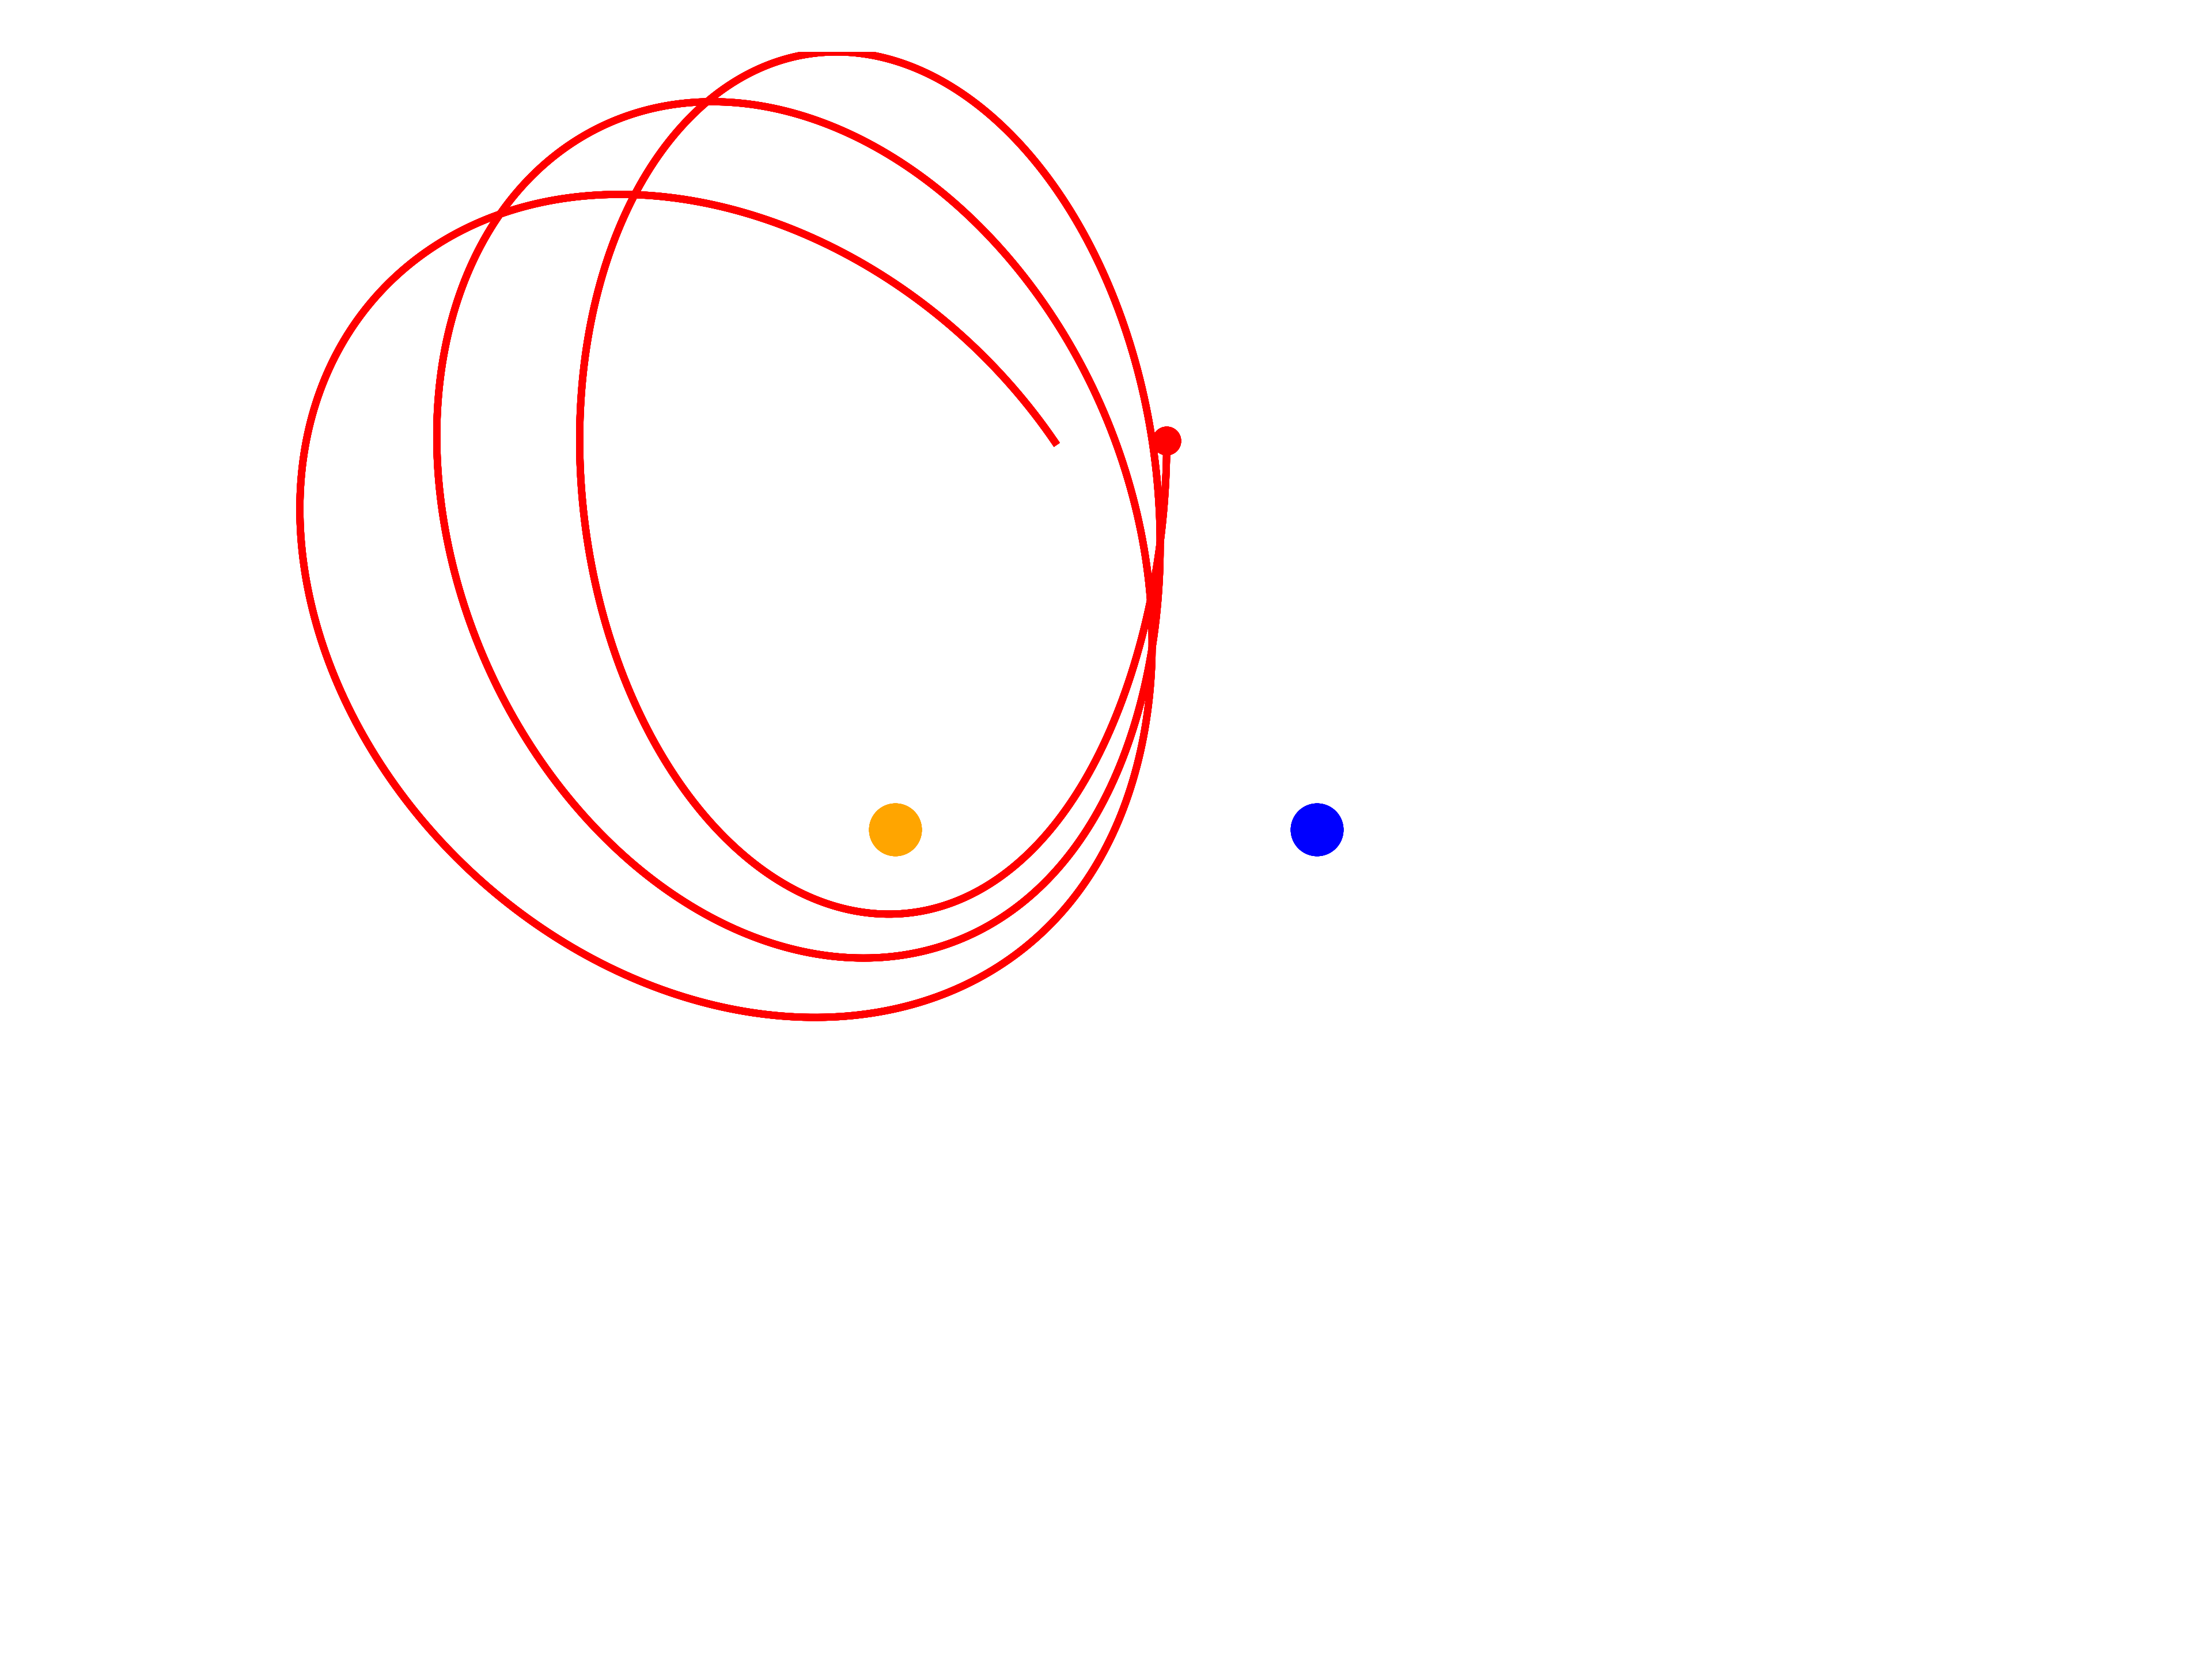
\includegraphics[scale=\myscale,scale=0.7,trim={1cm 3.5cm 5cm 0},clip]{figures/satellite-01.png}
  \quad
  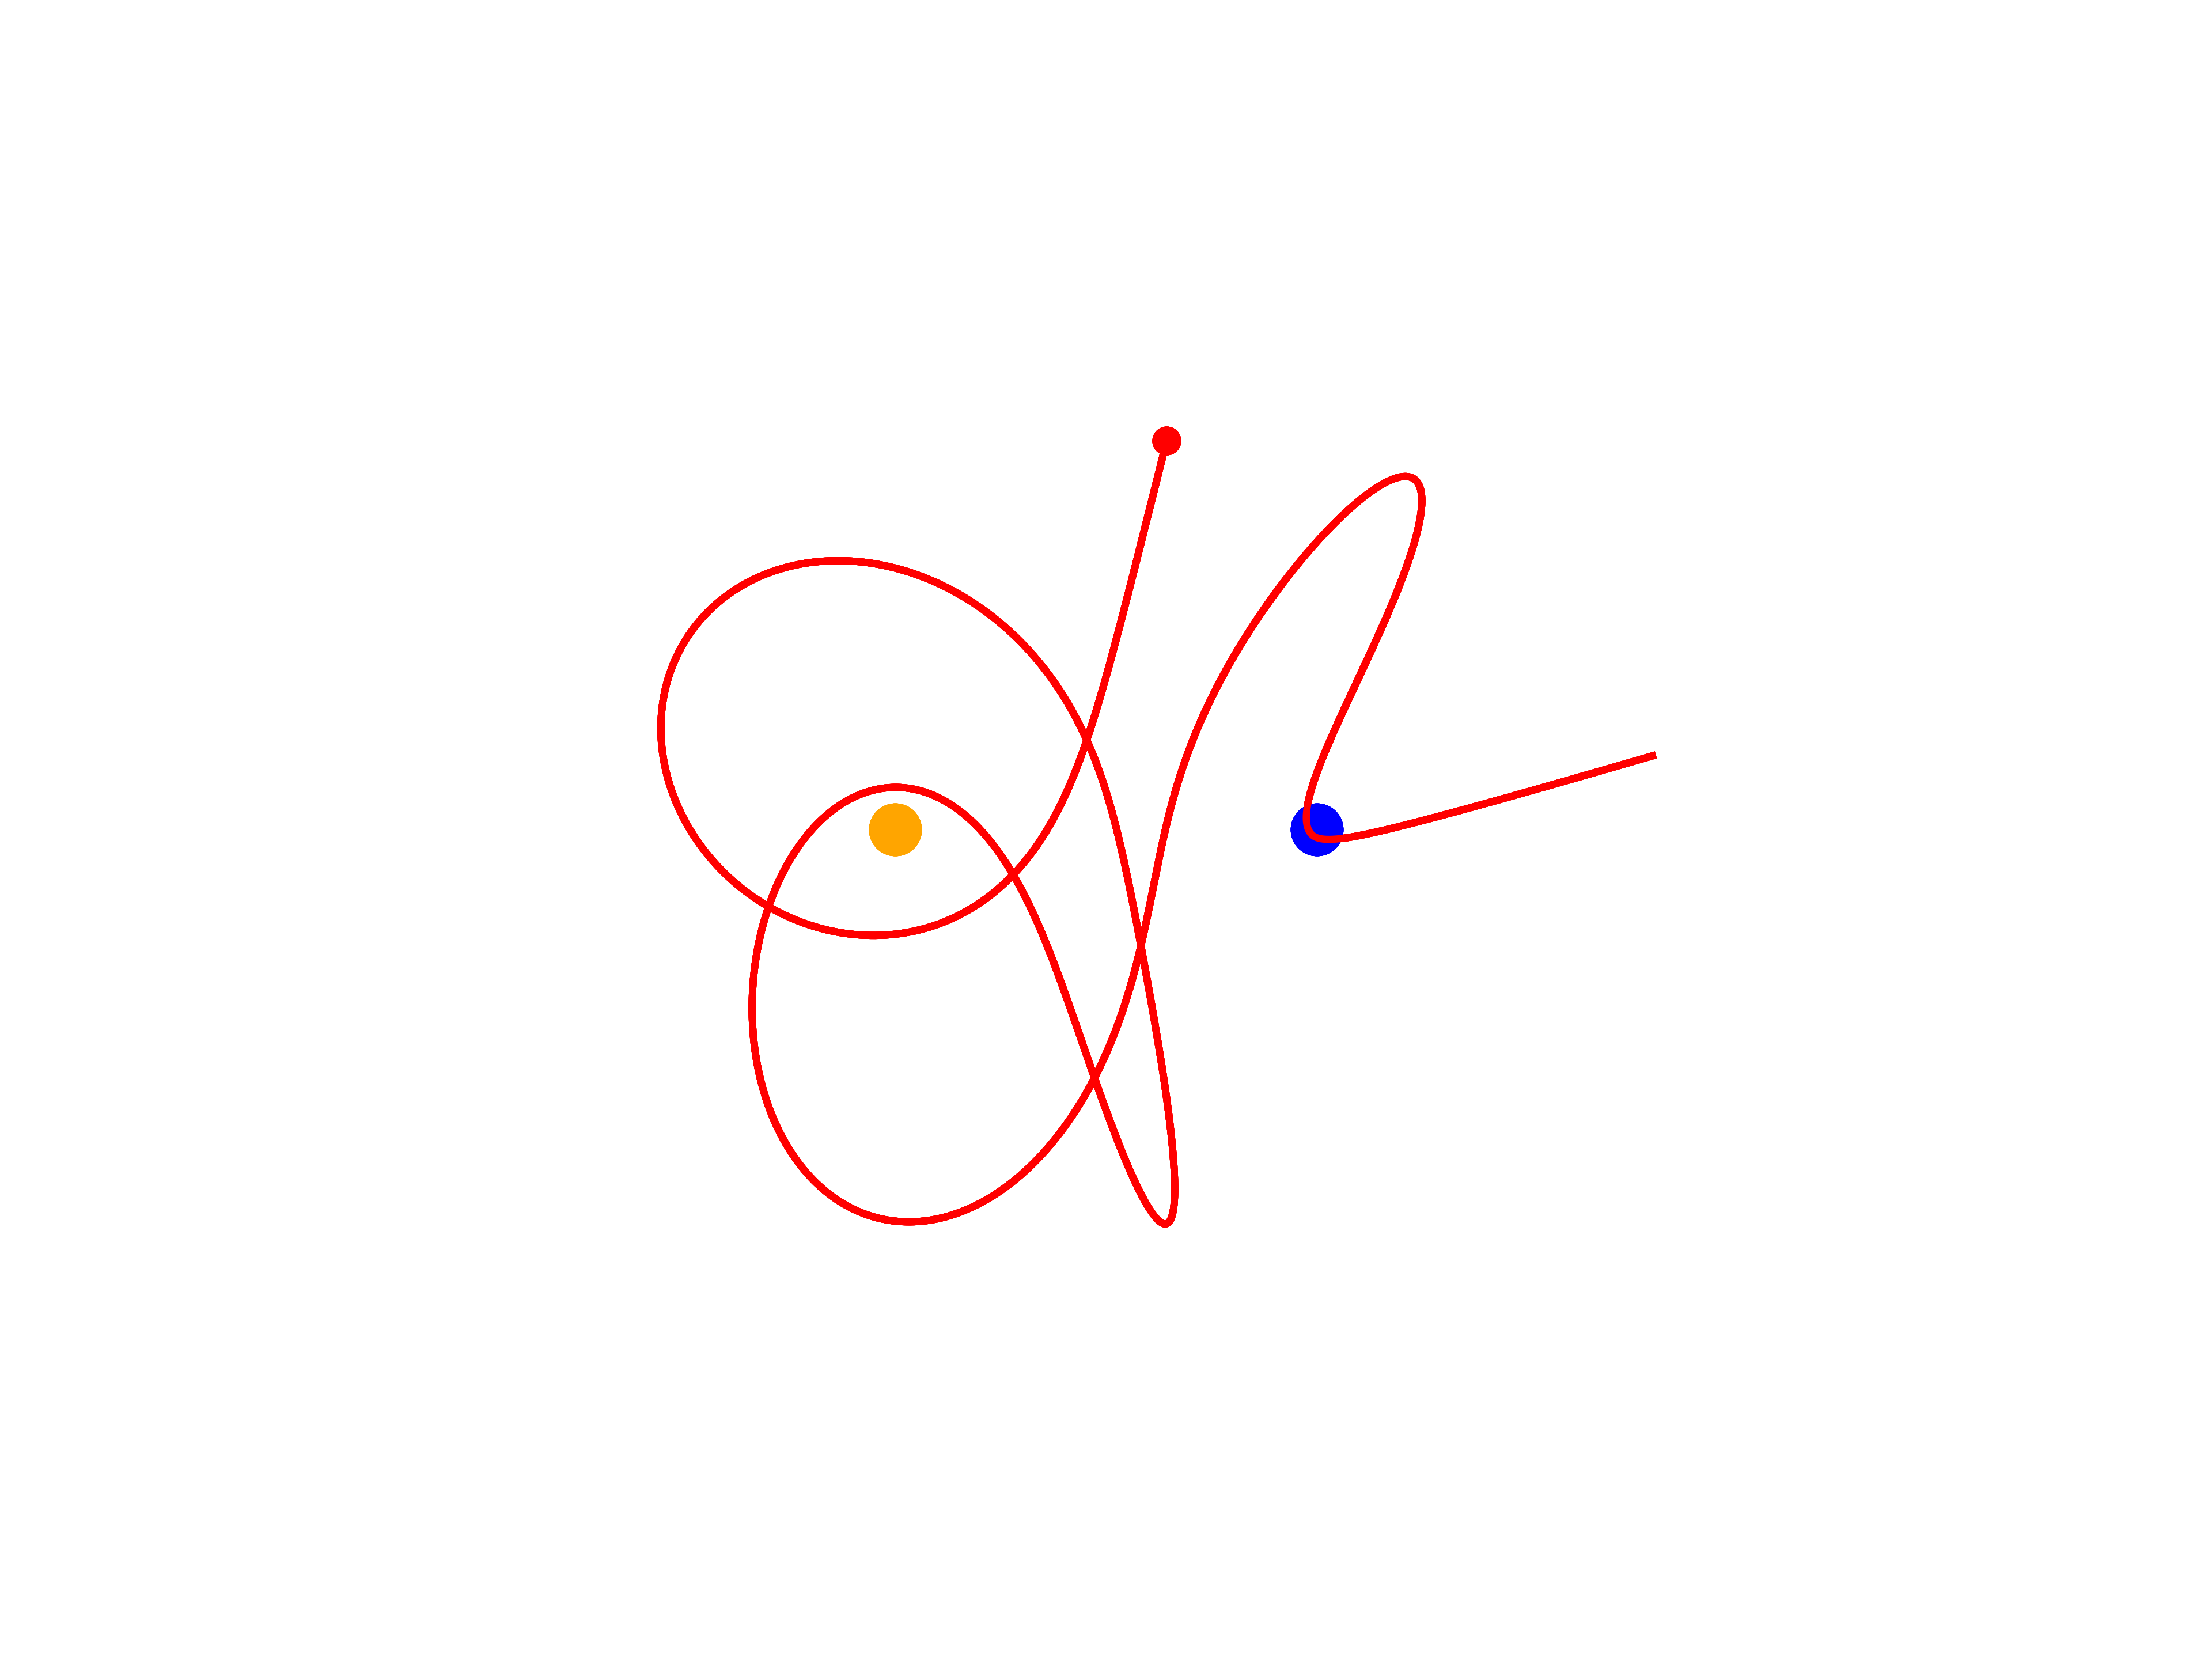
\includegraphics[scale=\myscale,scale=0.7,trim={2cm 2cm 2cm 3cm},clip]{figures/satellite-02.png}
\end{center}



\end{document}